\documentclass[12pt,twoside]{article}
\maxdeadcycles=1000 % Output loop---200 consecutive dead cycles.

\usepackage{paperlighter}

% Remove page numbering
%\pagenumbering{gobble}

\usepackage{longtable, setspace, outlines, tabularx}
 % for OliveGreen
\definecolor{OliveGreen}{rgb}{0,0.6,0}
% Set link colors
%\usepackage[rgb,dvipsnames]{xcolor}
%\hypersetup{colorlinks=true, linkcolor=RoyalBlue, urlcolor=RoyalBlue}

\usepackage{pdfpages} % for includepdf

\usepackage{selinput}
%\usepackage[margin=2cm]{geometry}
\usepackage{enumitem,varwidth}
%\usepackage[svgnames]{xcolor}
\usepackage{tikz} % for SWOT
\usetikzlibrary{shapes.geometric}

% Recommended, but optional, packages for figures and better typesetting:
\usepackage{microtype}
\usepackage{graphicx}
\usepackage{subfigure}
\usepackage{booktabs} % for professional tables

% Attempt to make hyperref and algorithmic work together better:
\newcommand{\theHalgorithm}{\arabic{algorithm}}


% For theorems and such
\usepackage{amsmath}
\usepackage{amssymb}
\usepackage{mathtools}
\usepackage{amsthm}

% if you use cleveref..
\usepackage[capitalize,noabbrev]{cleveref}

%%%%%%%%%%%%%%%%%%%%%%%%%%%%%%%%
% THEOREMS
%%%%%%%%%%%%%%%%%%%%%%%%%%%%%%%%
\theoremstyle{plain}
\newtheorem{theorem}{Theorem}[section]
\newtheorem{proposition}[theorem]{Proposition}
\newtheorem{lemma}[theorem]{Lemma}
\newtheorem{corollary}[theorem]{Corollary}
\theoremstyle{definition}
\newtheorem{definition}[theorem]{Definition}
\newtheorem{assumption}[theorem]{Assumption}
\theoremstyle{remark}
\newtheorem{remark}[theorem]{Remark}

% Todonotes is useful during development; simply uncomment the next line
%    and comment out the line below the next line to turn off comments
%\usepackage[disable,textsize=tiny]{todonotes}
\usepackage[textsize=tiny]{todonotes}

% Chinese
\usepackage{xeCJK} % for Chinese, compiling by XeLaTex
\usepackage{indentfirst}
\setlength{\parindent}{2em}  % setting the indentation to be two Chinese characters size.
\usepackage{fontspec} %設定字體
% Fandol font (the default)  not shown "內"
\setCJKmainfont{[Iansui094-Regular.ttf]}
\setCJKsansfont{[Iansui094-Regular.ttf]}
\setCJKmonofont{[Iansui094-Regular.ttf]}
%\setCJKmainfont{AR PL UMing TW MBE} % AR PL UMing TW MBE or "UKai" https://www.overleaf.com/learn/latex/Questions/Which_OTF_or_TTF_fonts_are_supported_via_fontspec%3F#Chinese
%BiauKai} %標楷體 from macOS %設定中文為系統上的字型,而英文不去更動,使用原TeX字型
%\setCJKmainfont[Vertical=RotatedGlyphs]{AR PL UMing TW MBE}


%%%%%%%%%%%%%
%% Chinese section numbering
%% by https://tex.stackexchange.com/questions/535650/customize-section-numbering-format-for-chinese-typesetting
%% answered Apr 1, 2020 at 13:10 wave
% https://tex.stackexchange.com/users/208733/wave

\usepackage{zhnumber}

\usepackage{titlesec}
\usepackage{titling}
%\usepackage{fontspec}
\usepackage{newunicodechar}
\usepackage{tocloft} % adding the tocloft package for toc customization

\setcounter{tocdepth}{5}
\setcounter{secnumdepth}{5}

% zhnum[style={Traditional,Financial}] doesn't work with the section counter,
% so we define our own counter and increase it every time in \thesection
\newcounter{mysec}[section]
\renewcommand\thesection{%
    \addtocounter{mysec}{1}%
    \zhnum[style={Traditional,digitals}]{mysec}、} % Financial
\renewcommand\thesubsection{(\zhnum{subsection})、} % added a 、
\renewcommand\thesubsubsection{(\zhnum{subsubsection})} % added parentheses
% (full-width, don't know if that's what you want)
\renewcommand\theparagraph{} % you don't want paragraph numbers
\renewcommand\thesubparagraph{} % nor subparagraph numbers

% we have to adjust the spacing in the toc because the section label is longer than usual
\addtolength\cftsecnumwidth{1em}
\addtolength\cftsubsecindent{1em}
\addtolength\cftsubsubsecindent{1em}

% here we need to make sure the normal section counter is accessed
\titleformat{\section}{\Large\bfseries\sffamily\filcenter}
    {\zhnum[style={Traditional,digitals}]{section}、}{.5em}{} % financial
% not really sure what you intend to achieve with \fontsize but I'll leave it here
\titleformat*{\subsection}{\bfseries\sffamily} %\fontsize{18}{20}
\titleformat*{\subsubsection}{\bfseries\sffamily} %\fontsize{16}{18}

% no extra version for numberless is necessary since no numbers are used anyways
% also you get newlines from omitting the [display] in \titleformat already
\titleformat{\paragraph}
    {\fontsize{14}{16}\bfseries\sffamily}{}{0em}{} 
\titleformat{\subparagraph}
    {\fontsize{12}{14}\bfseries\sffamily}{}{0em}{}
% we need the following so that they don't indent (second argument, 0em);
% you'll have to adjust the spacing though since this is not display style anymore:
\titlespacing*{\paragraph}{0em}{3.25ex plus 1ex minus .2ex}{.75ex plus .1ex} 
\titlespacing*{\subparagraph}{0em}{3.25ex plus 1ex minus .2ex}{.75ex plus .1ex}

\renewcommand{\maketitlehooka}{\sffamily}

\renewcommand{\baselinestretch}{1.2}
\renewcommand{\contentsname}{目錄} %{目次}

\usepackage{hyperref}
\hypersetup{
  colorlinks=true,
  linkcolor=[rgb]{0,0.37,0.53},
  citecolor=[rgb]{0,0.47,0.68},
  filecolor=[rgb]{0,0.37,0.53},
  urlcolor=[rgb]{0,0.37,0.53},
  % pagebackref=true, % this is ignored
  linktoc=all}

%\usepackage{hyperref}
% \usepackage[utf8x]{inputenc} do not use inputenc with XeTeX
% \usepackage{fixltx2e} not required any more

%\usepackage{rotating}

%%%%%%

\slimtitle{特需中心} %Paperlighter Example}
\slimauthor{萬芳醫院牙科部}


\begin{document} % 獎勵醫院提供特殊需求者牙科醫療服務
%衛生福利部
%111 年度「特殊需求者牙科醫療服務獎助計畫」 申請獎助作業規定
%本計畫經費財源為菸品健康福利捐,屬特定收入來源;年度進行中

%111年度「特殊需求者牙科醫療服務獎助計畫」計畫申請書

\thispagestyle{empty}

\lightertitle{
%\Large
\hspace{2.3cm} %臺北市立萬芳醫院牙科部
衛生福利部醫療發展基金獎助辦理

\hspace{0.6cm} 111年度「特殊需求者牙科醫療服務獎助計畫」

\hspace{5.6cm} 計畫申請書}
% 特殊需求者牙醫醫療服務
%居家牙醫醫療服務計畫
% 計畫申請書內容與格式
% 綜合資料表
% 進階照護院所:口腔醫療與保健推廣計畫書
\vspace{1.6cm}
\begin{figure}[H]
    \centering

\includegraphics[width=10cm]{MOHW_LOGO_0030101001.pdf}
\end{figure}
\vspace{2cm}

{\Large
計畫名稱: \underline{111年度「特殊需求者牙科醫療服務獎助計畫」}
\vspace{4mm}

執行單位: \underline{臺北市立萬芳醫院牙科部} %-委託財團法人私立臺北醫學大學辦理
\vspace{4mm}

計畫主持人: \underline{祁力行} \hspace{5cm} 職稱: \underline{特殊需求者口腔醫學科主任}
\vspace{1mm}

計畫聯絡人: \underline{張芝菱}
\vspace{4mm}

計畫執行期間: \underline{111年4月1日至12月31日}
}
\clearpage



%%
\lighterauthor{祁力行$^{\dagger}$, 李勝揚$^{\ddagger}$}

\lighteraddress{$^\dagger$}{臺北市立萬芳醫院牙科部口腔顎面外科}
\lighteraddress{$^\ddagger$}{臺北市立萬芳醫院牙科部}


\lighteremail{110255@w.tmu.edu.tw}
%110050@w.tmu.edu.tw}

% table of contents
\tableofcontents \clearpage

%\begin{abstract}
摘要:
「身心障礙者口腔照護指導員」訓練課程,多年的臨床工作,許多患者朋友從自行前來就醫,到現在由全家總動員推著輪椅來就醫,生活打理也漸漸需要他人代勞,甚至基本的口腔衛生照護,也面臨須由家人或照護者協助完成;平常在醫學中心,時常會有加護病房住院患者或化療患者牙科會診需求,臥床患者或這些有全身性疾病患者,經常面臨因口腔照護不佳造成牙痛或感染的困擾。

先申請特需中心,然後牙科部專任醫師才具有到宅牙醫服務的資格,當然也需要身障照護的學分。到宅小組需要一名醫師、一名護理師,攜帶必要設備,每一名案主收案都事先申請核可
%Using \LaTeX{} to write papers is concise and convenient. However, for writing in life, complicated \LaTeX{} style-files (e.g., elegantpaper) are difficult to access, or submission style-files (e.g., journal or conference) are not free indeed. To tackle these problems and satisfy an elegant and straightforward scientific writing, \textbf{paperlighter.sty}, a one-column style-file, is designed. This document is edited from icml2022.sty and provides a basic paper template. Compared to icml2022.sty, paperlighter.sty contain fewer operations, reducing adjustment while keep graceful. \textbf{\textit{Notably, the paper's main content only describes the format of icml2022.sty. We place the content to show the actual effect of paperlighter.sty.}}
\end{abstract} % no more
%
\section{Format of the Paperlighter}

Format of paperlighter is defined in this section.

\subsection{Dimensions}

The text of the paper has an
overall width of 6.75~inches, and height of 9.0~inches. The left margin should be 0.75~inches and the top
margin 1.0~inch (2.54~cm). The right and bottom margins will depend on
whether you print on US letter or A4 paper, but all final versions
must be produced for US letter size.

The paper body should be set in 10~point type with a vertical spacing
of 11~points. Please use Times typeface throughout the text.

\subsection{Title}

The paper title should be set in 14~point bold type and centered
between two horizontal rules that are 1~point thick, with 1.0~inch
between the top rule and the top edge of the page. Capitalize the
first letter of content words and put the rest of the title in lower
case.

\subsection{Author Information for Submission}
\label{author info}

Use \verb+\lighterauthor{...}+ to specify authors and \verb+\lighteraddress{...}+ to specify affiliations. (Read the TeX code used to produce this document for an example usage.) The author information
will not be printed unless \texttt{accepted} is passed as an argument to the
style file.

\subsection{Abstract}

The paper abstract should begin in the left column, 0.4~inches below the final
address. The heading `Abstract' should be centered, bold, and in 11~point type.
The abstract body should use 10~point type, with a vertical spacing of
11~points, and should be indented 0.25~inches more than normal on left-hand and
right-hand margins. Insert 0.4~inches of blank space after the body. Keep your
abstract brief and self-contained, limiting it to one paragraph and roughly 4--6
sentences. Gross violations will require correction at the camera-ready phase.

\subsection{Partitioning the Text}

You should organize your paper into sections and paragraphs to help
readers place a structure on the material and understand its
contributions.

\subsubsection{Sections and Subsections}

Section headings should be numbered, flush left, and set in 11~pt bold
type with the content words capitalized. Leave 0.25~inches of space
before the heading and 0.15~inches after the heading.

Similarly, subsection headings should be numbered, flush left, and set
in 10~pt bold type with the content words capitalized. Leave
0.2~inches of space before the heading and 0.13~inches afterward.

Finally, subsubsection headings should be numbered, flush left, and
set in 10~pt small caps with the content words capitalized. Leave
0.18~inches of space before the heading and 0.1~inches after the
heading.

Please use no more than three levels of headings.

\subsubsection{Paragraphs and Footnotes}

Within each section or subsection, you should further partition the
paper into paragraphs. Do not indent the first line of a given
paragraph, but insert a blank line between succeeding ones.

You can use footnotes\footnote{Footnotes
should be complete sentences.} to provide readers with additional
information about a topic without interrupting the flow of the paper.
Indicate footnotes with a number in the text where the point is most
relevant. Place the footnote in 9~point type at the bottom of the
column in which it appears. Precede the first footnote in a column
with a horizontal rule of 0.8~inches.\footnote{Multiple footnotes can
appear in each column, in the same order as they appear in the text,
but spread them across columns and pages if possible.}

\begin{figure}[ht]
\vskip 0.2in
\begin{center}
\centerline{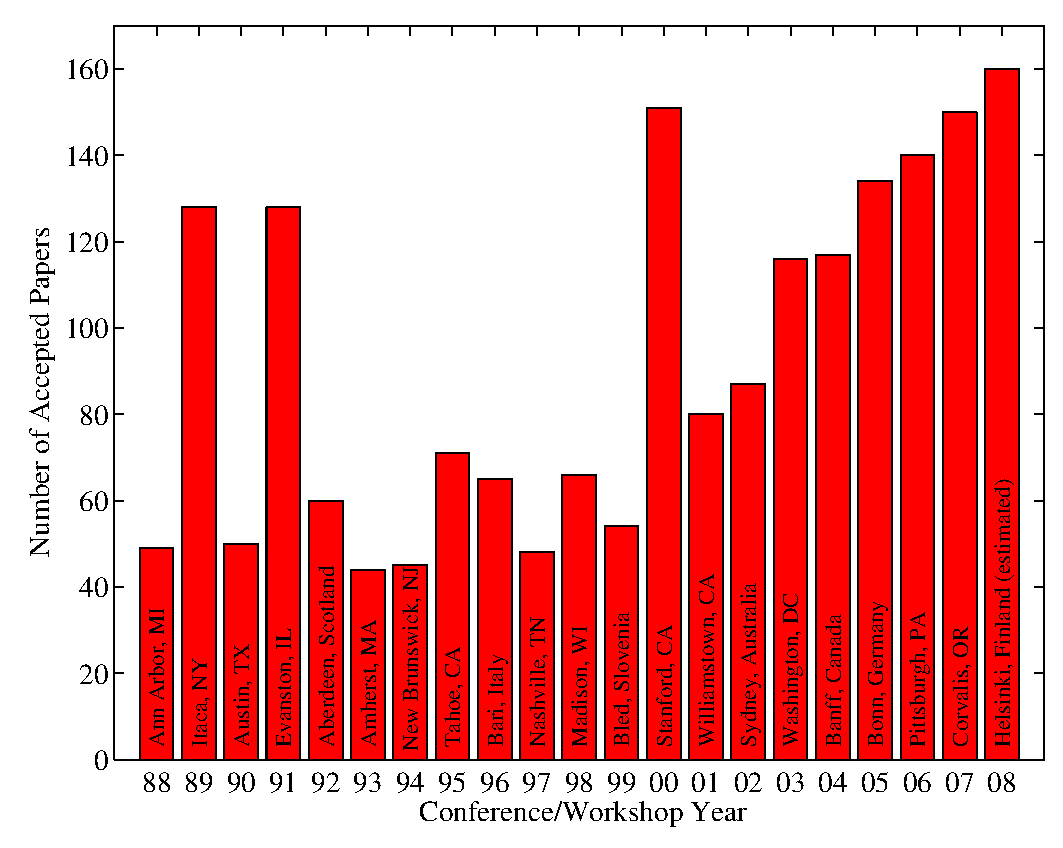
\includegraphics[width=\columnwidth]{figure/icml_numpapers.eps}}
\caption{Historical locations and number of accepted papers for International
Machine Learning Conferences (ICML 1993 -- ICML 2008) and International
Workshops on Machine Learning (ML 1988 -- ML 1992). At the time this figure was
produced, the number of accepted papers for ICML 2008 was unknown and instead
estimated.}
\label{icml-historical}
\end{center}
\vskip -0.2in
\end{figure}

\subsection{Figures}

You may want to include figures in the paper to illustrate
your approach and results. Such artwork should be centered,
legible, and separated from the text. Lines should be dark and at
least 0.5~points thick for purposes of reproduction, and text should
not appear on a gray background.

Label all distinct components of each figure. If the figure takes the
form of a graph, then give a name for each axis and include a legend
that briefly describes each curve. Do not include a title inside the
figure; instead, the caption should serve this function.

Number figures sequentially, placing the figure number and caption
\emph{after} the graphics, with at least 0.1~inches of space before
the caption and 0.1~inches after it, as in
\cref{icml-historical}. The figure caption should be set in
9~point type and centered unless it runs two or more lines, in which
case it should be flush left. You may float figures to the top or
bottom of a column, and you may set wide figures across both columns
(use the environment \texttt{figure*} in \LaTeX). Always place
two-column figures at the top or bottom of the page.

\subsection{Algorithms}

If you are using \LaTeX, please use the ``algorithm'' and ``algorithmic''
environments to format pseudocode. These require
the corresponding stylefiles, algorithm.sty and
algorithmic.sty, which are supplied with this package.
\cref{alg:example} shows an example.

\begin{algorithm}[tb]
   \caption{Bubble Sort}
   \label{alg:example}
\begin{algorithmic}
   \STATE {\bfseries Input:} data $x_i$, size $m$
   \REPEAT
   \STATE Initialize $noChange = true$.
   \FOR{$i=1$ {\bfseries to} $m-1$}
   \IF{$x_i > x_{i+1}$}
   \STATE Swap $x_i$ and $x_{i+1}$
   \STATE $noChange = false$
   \ENDIF
   \ENDFOR
   \UNTIL{$noChange$ is $true$}
\end{algorithmic}
\end{algorithm}

\subsection{Tables}

You may also want to include tables that summarize material. Like
figures, these should be centered, legible, and numbered consecutively.
However, place the title \emph{above} the table with at least
0.1~inches of space before the title and the same after it, as in
\cref{sample-table}. The table title should be set in 9~point
type and centered unless it runs two or more lines, in which case it
should be flush left.

% Note use of \abovespace and \belowspace to get reasonable spacing
% above and below tabular lines.

\begin{table}[t]
\caption{Classification accuracies for naive Bayes and flexible
Bayes on various data sets.}
\label{sample-table}
\vskip 0.15in
\begin{center}
\begin{small}
\begin{sc}
\begin{tabular}{lcccr}
\toprule
Data set & Naive & Flexible & Better? \\
\midrule
Breast    & 95.9$\pm$ 0.2& 96.7$\pm$ 0.2& $\surd$ \\
Cleveland & 83.3$\pm$ 0.6& 80.0$\pm$ 0.6& $\times$\\
Glass2    & 61.9$\pm$ 1.4& 83.8$\pm$ 0.7& $\surd$ \\
Credit    & 74.8$\pm$ 0.5& 78.3$\pm$ 0.6&         \\
Horse     & 73.3$\pm$ 0.9& 69.7$\pm$ 1.0& $\times$\\
Meta      & 67.1$\pm$ 0.6& 76.5$\pm$ 0.5& $\surd$ \\
Pima      & 75.1$\pm$ 0.6& 73.9$\pm$ 0.5&         \\
Vehicle   & 44.9$\pm$ 0.6& 61.5$\pm$ 0.4& $\surd$ \\
\bottomrule
\end{tabular}
\end{sc}
\end{small}
\end{center}
\vskip -0.1in
\end{table}

Tables contain textual material, whereas figures contain graphical material.
Specify the contents of each row and column in the table's topmost
row. Again, you may float tables to a column's top or bottom, and set
wide tables across both columns. Place two-column tables at the
top or bottom of the page.

\subsection{Theorems and such}
The preferred way is to number definitions, propositions, lemmas, etc. consecutively, within sections, as shown below.
\begin{definition}
\label{def:inj}
A function $f:X \to Y$ is injective if for any $x,y\in X$ different, $f(x)\ne f(y)$.
\end{definition}
Using \cref{def:inj} we immediate get the following result:
\begin{proposition}
If $f$ is injective mapping a set $X$ to another set $Y$, 
the cardinality of $Y$ is at least as large as that of $X$
\end{proposition}
\begin{proof} 
Left as an exercise to the reader. 
\end{proof}
\cref{lem:usefullemma} stated next will prove to be useful.
\begin{lemma}
\label{lem:usefullemma}
For any $f:X \to Y$ and $g:Y\to Z$ injective functions, $f \circ g$ is injective.
\end{lemma}
\begin{theorem}
\label{thm:bigtheorem}
If $f:X\to Y$ is bijective, the cardinality of $X$ and $Y$ are the same.
\end{theorem}
An easy corollary of \cref{thm:bigtheorem} is the following:
\begin{corollary}
If $f:X\to Y$ is bijective, 
the cardinality of $X$ is at least as large as that of $Y$.
\end{corollary}
\begin{assumption}
The set $X$ is finite.
\label{ass:xfinite}
\end{assumption}
\begin{remark}
According to some, it is only the finite case (cf. \cref{ass:xfinite}) that is interesting.
\end{remark}
%restatable

\subsection{Citations and References}

If you rely on the \LaTeX{} bibliographic
facility, use \texttt{natbib.sty}
included in the style-file package to obtain reference.

Citations within the text should include the authors' last names and
year. If the authors' names are included in the sentence, place only
the year in parentheses, for example when referencing Arthur Samuel's
pioneering work \yrcite{Samuel59}. Otherwise place the entire
reference in parentheses with the authors and year separated by a
comma \cite{Samuel59}. List multiple references separated by
semicolons \cite{kearns89,Samuel59,mitchell80}. Use the `et~al.'
construct only for citations with three or more authors or after
listing all authors to a publication in an earlier reference \cite{MachineLearningI}.

Use an unnumbered first-level section heading for the references, and use a
hanging indent style, with the first line of the reference flush against the
left margin and subsequent lines indented by 10 points. The references at the
end of this document give examples for journal articles \cite{Samuel59},
conference publications \cite{langley00}, book chapters \cite{Newell81}, books
\cite{DudaHart2nd}, edited volumes \cite{MachineLearningI}, technical reports
\cite{mitchell80}, and dissertations \cite{kearns89}.

Alphabetize references by the surnames of the first authors, with
single author entries preceding multiple author entries. Order
references for the same authors by year of publication, with the
earliest first. Make sure that each reference includes all relevant
information (e.g., page numbers).

Please put some effort into making references complete, presentable, and
consistent, e.g. use the actual current name of authors.
If using bibtex, please protect capital letters of names and
abbreviations in titles, for example, use \{B\}ayesian or \{L\}ipschitz
in your .bib file.
%{
%一、計畫書封面:至少包含計畫名稱(包含計畫執行地區)、計畫執行單位、計 畫執行期間。
%二、書寫格式:以 word 建檔,A4 版面,由左而右,由上而下,標楷體 14 號字 型,橫式書寫,填寫綜合資料表,另計畫書編有目錄頁碼。

%三、計畫本文至少應包括: (一)緣起/前言:請敘述申請本計畫產生之背景。 
%(二)現況分析:請敘述現實施地區所呈現問題。 
%(三)計畫人力配置:組織架構、現況、醫事人力、醫療設備、經營現況;另詳述醫事人力(專任或兼任醫師、執業登錄)及參與獎助服務醫師名冊 並檢附受有 10 學分以上身心障礙相關教育訓練之證明文件(僅需列出指 定課程 10 個學分數,並完整確實標註清楚)。

%(四)計畫內容: 
%1、目的。
%2、計畫執行期程、申請之獎助項目及預估獎勵金額。
%3、依序撰寫各項預定辦理內容與進行步驟。
%4、過去 3 年計畫執行情形及未來 3 年執行目標、摘要表(如附件 1、6)、衛生局指定辦理身心障礙者特別門診之資格證明文件(如公文,並得為影、複本)。
%5、品質和成效。 
%6、預期效益。

%(五)後續發展或推廣:詳述計畫執行結束後之後續規劃,以達獎助後之永續責任,並可嘗試建立標準模式,提供其他地區標竿參考。

%}
% 口腔醫療與保健推廣及保健推廣計畫書
% 僅第一項: 補助醫院提供特殊需求者牙科醫療服務
\section{緣起}
臺北市立萬芳醫院牙科部設置特殊需求者牙科門診(以下稱特需中心),每週門診2診次,專門服務身心障礙者,牙科櫃台附有身心障礙服務窗口,設置志工,與負責身心障礙門診之牙科輔助人員共同幫忙引導、溝通、協助患者就醫。候診區及初診區均有輪椅無障礙空間。
%先申請特需中心,然後牙科部專任醫師才具有到宅牙醫服務的資格,當然也需要身障照護的學分。到宅小組需要一名醫師、一名護理師,攜帶必要設備,每一名案主收案都事先申請核可
特殊需求者的口腔照護,因日常生活打理由照顧者代勞,往往無法顧及基本的口腔衛生照護,行動不便、甚至長期在宅臥床的患者更面臨齲齒、牙周病細菌感染的重大危機,因其就醫之阻礙甚多,四、五層樓之公寓往往沒有電梯。口腔細菌感染有機會吸入造成肺炎感染,增加患者身體的負擔。
萬芳醫院牙科部特需中心,配合長照2.0政策,除服務原有的到院病患,更自111年3月起進一步籌備居家牙醫醫療服務(以下稱到宅牙醫)。

\section{現況分析}
身心障礙者特別門診,每週開設2診(週四下午陳培惠醫師、週六上午謝承祐醫師)。家庭牙醫科陳醫師,及兒童牙科謝醫師,均已接受30學分身心障礙教育訓練。除執行適當的口腔與牙齒治療,並對患者與其陪同家人進行口腔保健教育。110年共計服務人次300人,個案管理追蹤人數60名。
	
%「全民健康保險會」協定年度醫療給付費用總額事項」辦理
% https://www.nhi.gov.tw/BBS_Detail.aspx?n=73CEDFC921268679&sms=D6D5367550F18590&s=DC5108C6E3DD21D0

本院牙科部依據「111年全民健康保險牙醫門診總額特殊醫療服務計畫」,辦理「特殊需求者到宅牙醫計畫」,旨在擴大特定身心障礙者口腔醫療與保健推廣。預計每年可穩定服務(每名患者每2個月一次)20名以上的居家醫療需求者。
%(以下稱本計畫)。

\section{計畫人力配置}

\subsection{組織架構}
\begin{outline}

%\1 組織架構
\1 現況: 萬芳醫院牙科部,「特殊需求者口腔醫學科」籌備處,規畫整合原有特需門診,加上到宅牙醫服務,形成完整的特需服務與衛生教育推廣網絡
\1 醫事人力: %詳述醫事人力(專任或兼任醫師、執業登錄)及參與獎助服務醫師名冊並檢附受有 10 學分以上身心障礙相關教育訓練之證明文件(僅需列出指定課程10個學分數,並完整確實標註清楚)。
本院專任醫師三名,口腔顎面外科主任祁力行醫師、
家庭牙醫科主任陳培惠醫師、
兒童牙科主任謝承祐醫師,均已接受30學分身心障礙教育訓練。並領有ACLS高等心臟急救訓練合格證書。特殊需求牙科護士一名。
\end{outline}

\subsection{醫療設備}

\begin{outline}
\1 無障礙空間及設施
\1 個人防護,遵循感染控制標準流程
\1 牙科X光機、牙科診療椅
\1 家庭牙醫、兒童牙科及口腔顎面外科門診裝備,如洗牙機、強力抽吸設備與抽痰管、牙科治療器械、開口器、中醫雷射針灸
\1 生理監測器(血壓、血氧)
\1 急救車(心電圖、心臟電擊器),急救藥品(定期盤點控管)、急救設備(喉頭鏡、人工氣道氣管內管)、氧氣設備(壁式氧氣、節流裝置、氧氣面罩、潮氣瓶)
\end{outline}

\subsection{經營現況}

\begin{outline}
\1 每週開設2診(週四下午陳醫師照護成人、週六上午謝醫師照護18歲以下特需病患)
\1 執行口腔與牙齒治療,並對患者與其陪同家人進行口腔保健教育
\1 110年共計服務人次300人,個案管理追蹤人數60名
\end{outline}


\section{計畫內容}

\subsection{目的}
配合衛生福利部政策,推動「身心障礙牙科醫療服務網絡模式」雙向轉診,提供特殊需求者牙科醫療服務,以及口腔衛生保健雙向互動。


\subsection{計畫執行期程}
111年4月1日至12月31日

\subsection{獎助項目}
提供特殊需求者牙科醫療服務

\subsection{預估獎勵金額}
\begin{outline}
\1 計畫期間達成基本應辦理事項,請領獎勵費用計新臺幣(以下同)38萬元整
\1 每周開設特別門診3診,與8家醫療機構(其中3家需為未合作過之新增名單)建置轉診機制,另請領獎勵費用計5萬元整
\1 共計43萬元整
\end{outline}

\subsection{計畫期間辦理事項}
%依序撰寫各項預定辦理內容與進行步驟}

\begin{outline}
\1 每週開設特別門診3診(每診至少3小時)
    \2 週一上午祁力行醫師,到宅牙醫服務(特殊需求牙科負責護士陪同)
    \2 週三上午祁力行醫師(口腔顎面外科,備有雷射針灸)
    \2 週四下午陳培惠(家庭牙科)照護成人特需病患
    \2 週六上午謝承祐(兒童牙科)照護18歲以下特需病患
    
\1 進行口腔衛生教育,指導患者及其照顧家人
    \2 衛教人員由醫師及特殊需求牙科負責護士擔任
    \2 衛教內容包括心理建設、臉部減敏按摩、中醫穴道按摩、吞嚥練習、舌頭運動、牙齒清潔(小牙刷)及牙縫清潔(牙線棒、牙間刷)
    \2 衛教工作詳實紀錄於特殊需求者口腔衛教照護衛教紀錄表(如附件2-1)
    
\1 個案追蹤管理
    \2 由特殊需求牙科負責護士擔任
    \2 針對特殊需求者患者,於治療與衛教後次日,進行個案追蹤管理工作,詢問術後情況、口腔清潔狀況,安排並鼓勵每二個月定期回診/到宅
    \2 建立「病友」LINE群組,回傳照片、錄製影片加強衛教宣導
    \2 製作個案追蹤管理紀錄表(如附件2-2、2-3)

\1 身心障礙牙科醫療服務網絡模式
    \2 臺北市文山區已有14家身心障礙牙科醫療服務院所
    \2 於計畫期間至少與8家院所建立並簽具合作契約書
    \2 主動與臺北市衛生局及臺北市牙醫師公會,會商建置區域內特殊需求者醫療轉診制度,增進合作醫院間交流活動
    \2 特殊需求者牙科醫療服務轉介單如附件2-4

\1 特需者口腔保健衛教講座
    \2 與身心障礙福利機構、特殊教育機構或特教班、聯合評估中心或發展遲緩療育機構、老人福利機構、長照機構或身心障礙團體等合作
    \2 舉辦6場講座,提供口腔保健衛教、口腔檢查,視該機構情況亦可能安排簡單診療服務(超音波洗牙、塗氟)
    \2 定期到萬芳醫院12樓護理之家,進行口腔保健衛教、口腔檢查,及簡單診療服務(拔牙、超音波洗牙、塗氟)
    \2 指導牙科PGY醫師進行社區服務
    
\1 特殊需求者牙科醫療培訓計畫
    \2 安排學員參加特殊需求者牙科醫療服務示範中心(如,臺大醫院、雙和醫院)舉辦之牙醫師培訓計畫
    \2 每年1名牙科部PGY醫師完成訓練,且領有證書
    \2 每週一上午到宅牙醫服務,由祁力行醫師、特殊需求牙科負責護士,帶領PGY醫師出診
    
\1 特殊需求者牙科醫療服務季報表
    \2 定期於111年4月15日、7月15日、10月15日及112年1月6日,以電子郵件方式回報
    \2 服務累計表(季報表)如附件3


\end{outline}

\subsection{回顧與展望}
\begin{outline}
\1 萬芳醫院牙科部,過去3年計畫執行情形及未來3年執行目標(附件1)
\1 計畫期間辦理事項摘要表(附件16)
\1 111年04月開辦到宅牙醫服務
\end{outline}
%衛生局指定辦理身心障礙者特別門診之資格證明文件(如公文,並得為影、複本)。

%服務人次:
%係特定障礙類別之特殊需求者,於本計畫獎助之醫院,接受具 10 學分以上身心障礙相關教育訓練之醫師所提供之牙科醫療服務人次總數(不限其接受診療時間是否為特別門診時段),惟不含該病人當次僅接受口腔健康狀況檢查、塗氟、特定或非特定局部治療、全身麻醉評估、開藥、抽血、X 光、拆線、全身麻醉回診、特殊牙周疾病基本控制處置、口腔衛教、查看傷口、拔牙回診...等處置者。

\subsection{品質和成效}

\subsection{預期效益}


\section{後續發展或推廣}
\subsection{特殊需求者口腔醫學專科訓練}
臺灣特殊需求者口腔醫學會專科醫師
詳述計畫執行結束後之後續規劃,以達獎助後之永續責任

【110學年度 台大醫院 特殊需求者牙科醫療服務示範中心第三年住院醫師招募】
1 訓練特色
1.1 以特殊需求者為照護對象:特需牙科的病人範疇包含身心障礙牙科、醫院牙科、老人牙科、長期口腔照護牙科、早期療育牙科五大區塊。從自閉症的孩童到阿茲海默症的老人等等都是我們看診的病人,範圍非常廣泛,長期的回診追蹤的老病人也非常多。訓練內容包含特殊需求者之牙體復形、根管治療、牙周治療、包含智齒與多生牙在內的恆牙拔牙、全口或局部假牙製作等全人醫療照護。此外,訓練醫師亦可以在實際看診、醫科科外訓練與病例討論會議中更深入了解各種疾病的相關醫療知識與緊急處理流程,將來看任何病人(不是只有特殊需求者)都能臨危不亂,處理得宜。
1.2 醫科科外訓練:除了在特需牙科的訓練之外,也會安排醫科的科外訓練,到麻醉科、心臟內外科、兒童ICU病房、復健科、兒童心智科、基因醫學科等各科部進行學習,對各種系統性疾病有更近一步的認知,並運用於實際看診的病人上。
1.3 國外進修:本科之訓練醫師可以申請至美國加州大學洛杉磯分校(UCLA)牙醫學院進行為期兩個月的進修,以精進醫院牙科(Hospital dentitstry)為主的學術交流。
1.4 麻醉手術實際操作:本科訓練醫師每週都會安排全身麻醉以及鎮靜麻醉的手術得以親自操作完成治療,並收集專科訓練案例。週五早上的麻醉科聯合晨會以及科外麻醉科的訓練,都可以讓受訓住院醫師增進手術相關的知識與技術,可以順利與麻醉醫師溝通,對於麻醉手術能更得心應手。
1.5 笑氣麻醉操作與數位口掃:受訓醫師可以學習並操作笑氣鎮靜麻醉,得以應用於懼怕就診的病人上,也能帶領實習醫學生學習笑氣麻醉的操作技巧。數位口掃印模亦能運用於臨床,降低病人不適感,提高治療品質。
1.6 可依興趣選擇台大牙科其他專科,進行第二專長訓練。
1.7 交通好便利、生活真方便:北車、捷運站、機場捷運線,交通便利,餐廳多元。
1.8 完訓後可以申請台大特需牙科兼任主治醫師職位。
2 臨床時數與Loading
2.1 第三年起之住院醫師不用值班,沒有夜診,六日也沒有上班。例假日依照醫院標準放假。
2.2 平日早午診上班,算入勞基法上班時數。
2.3 臨床人力充足,助理與護理師可以提供四手到六手操作。
3 其他福利
3.1 有年終獎金、生日、三節獎金。
3.2 提供台大醫院宿舍,雙人房(1500元)及四人房(1000元)。
3.3 年假依照勞基法。
4 未來發展
4.1 訓練特殊需求者及一般患者全人照護醫療
4.2 醫科相關科外訓練
4.3 全身麻醉與鎮靜麻醉牙科治療訓練
4.4 完訓後可以申請台大特需牙科兼任主治醫師職位
4.5不會被強迫只能看特需病人,而是超級GP,兼具口外,兒牙能力


\subsection{到宅牙醫標準模式}
並可嘗試建立標準模式,提供其他地區標竿參考。



% my project main text
%% SWOT: Streghts, Weaknesses, Opportunities, Threats
% https://gist.github.com/ricardogarfe/4563453


\section{SWOT Matrix - \emph{(Strengths, Weaknesses, Opportunities, Threats)}}

% pentagon -> hexagon
\begin{tikzpicture}[
    hexagon/.style={%
        shape=regular polygon, regular polygon sides=6, minimum size=7.3cm, inner
        sep=-1mm, draw, fill=gray!10 %DarkSeaGreen!75!yellow
    }, font=\scriptsize\sffamily, thick
]

% \draw[help lines] (-16,-16) grid (16,16);
\filldraw[thin,gray,fill=gray!25] (-8,-8) rectangle (8,8);
\filldraw[thin,gray,fill=white] (-7.15,-7.15) rectangle (7.15,7.15);
\draw[thin,gray] (7.15,7.15)--(8,8) (-7.15,7.15)--(-8,8) (-7.15,-7.15)--(-8,-8)
(7.15,-7.15)--(8,-8);

% Strengths
% pentagon
\draw[thin, green] (-0.025,0.025)--(-7.05,0.025)--(-0.025,7.05)--cycle;

%\node[pentagon ,rotate=45] 
%\polygon[rotate=45]{6} 
\node[hexagon, rotate=45] at (-3.75,3.75) {
    \begin{varwidth}{\linewidth}
        \begin{itemize}[leftmargin=*,noitemsep]
            \item 社會責任與醫院評鑑
            %Technical and business expertise
            \item 守護文山新店深坑地區 %Domestic market orientation
            \item 偏鄉服務及特需中心 %初級
            %Stable management team
            \item 牙科部財務健全
            %Financial stability
            %\item Acquisition capabilities            
            \item 資深特需師資(四位) %七年30學分終身會員 %Economies of scale
            \item 複製北醫附醫五年到宅經驗 %Training programs
            %\item Loyalty and retention
        \end{itemize}
    \end{varwidth}
};
\draw (-2,2) node[rotate=45] {\large\textbf{Strengths}};

% Weaknesses
\draw[thin, brown!20!red] (0.025,0.025)--(7.05,0.025)--(0.025,7.05)--cycle;
\node[hexagon,rotate=-45] at (3.75,3.75) {
    \begin{varwidth}{\linewidth}
        \begin{itemize}[leftmargin=*,noitemsep]
            \item 初期經費與設備投資 %Centralized decisions
            \item  醫師、專責護士與人力規畫 %Accounts cross-selling
            \item 到宅牙醫行政文書
             %Marketing capabilities
            %\item 到宅醫療收入與時間成本 %Win on price image
            %\item 到宅交通費用 %BPO market
            %\item 特需案例來源
            %\item No differentiation
        \end{itemize}
    \end{varwidth}
};
\draw (2,2) node[rotate=-45] {\large\textbf{Weaknesses}};

% Opportunities
\draw[thin, green!50!blue] (-0.025,-0.025)--(-7.05,-0.025)--(-0.025,-7.05)--cycle;
%135
\node[hexagon,rotate=-45] at (-3.75,-3.75) {
    \begin{varwidth}{\linewidth}
        \begin{itemize}[leftmargin=*,noitemsep]
            \item  原PGY醫師(1人/月)支援連江縣立醫院 %Marketing push
            \item =>社區牙科訓練改為到宅牙醫服務 %Adding BPO capabilities
            \item 招募護士加入排班 %到宅醫師(二名排班) \item 到宅護士(二名排班)
            \item 牙科部祕書兼到宅牙醫行政
            \item 收取交通費/院方公務車支援 %Pricing structure
            \item 案例來源: 社區醫療部、出院準備服務 %Business process approach
            %\item %Annuity engagement
        \end{itemize}
    \end{varwidth}
};
\draw (-2,-2) node[rotate=-45] {\large\textbf{Opportunities}};

% Threats
\draw[thin, brown] (0.025,-0.025)--(7.05,-0.025)--(0.025,-7.05)--cycle;
\node[hexagon,rotate=45] at (3.75,-3.75) {
    \begin{varwidth}{\linewidth}
        \begin{itemize}[leftmargin=*,noitemsep]
            \item 到宅醫療收入不敷時間成本 %Profitability losses
            \item 收取到宅交通費形成門檻 %BPO market
            \item 特需案例來源
            
            %\item High-risk deals
            %\item Image change inability
            %\item Degree of automation
        \end{itemize}
    \end{varwidth}
};
\draw (2,-2) node[rotate=45] {\large\textbf{Threats}};
%
\draw(0,-7.55) node {\Large EXTERNAL};
\draw(0,7.55) node {\Large INTERNAL};
\draw(-7.55,0) node[rotate=90] {\Large POSITIVE};
\draw(7.55,0) node[rotate=270] {\Large NEGATIVE};
\draw[green](-0.6,0.6) node {\Huge\textbf{S}}; 
\draw[brown!20!red](0.6,0.6) node {\Huge\textbf{W}};
\draw[green!50!blue](-0.6,-0.6) node {\Huge\textbf{O}};
\draw[brown](0.6,-0.6) node {\Huge\textbf{T}};
\end{tikzpicture}
  
  % treatment planning
% U:如何善用每個優勢? (How can we Use each Strength?)
%S:如何停止每個劣勢? (How can we Stop each Weakness?)
%E:如何成就每個機會? (How can we Exploit each Opportunity?)
%D:如何抵禦每個威脅? (How can we Defend against each Threat?)

\begin{outline}

% 零基預算 Zero-based budgeting system
% 成本中心
\0 經費概算:
\1 人事(聘用人力學經歷) %Required staffing to complete department functions; What staffing would be required at what experience levels & salaries
\1 設備 %Required equipment/software/hardware necessary to complete the function
\1 出診交通費 %Required overhead costs needed to complete the function
\1 耗材 %Required overhead costs needed to complete the function
\1 教育訓練
\1 衛教宣導

\0 預期效益及效益指標(key performance index, KPI) %Current marketing efforts and their efficiency
\1 每週出診數、人次
\2 健保收入,交通費收入。轉診加成?
%(一)	預計提供高負荷家庭照顧者個案服務○○○人。
\2 每年預計提供宅照顧技巧○○人/○○人次
\1 每年預計辦理長照家庭照顧者之長照知識或照顧技能訓練○○○場,服務○○人及○○人次

%(四)	預計拓展○○照顧資訊小站、○○照顧支持小站。
%(五)	預計辦理○○場教育訓練,受益人數為○○人次。
\1 預計辦理○○場宣導活動,擴及人數為○○人次

\end{outline}

2022年籌備期程(Gantt chart)\\
\begin{tabular}{|c|cccc|}
\hline
 工作項目 & 四月 & 五月  & 六月 & 七月  \\
\hline
 聘用護理人員    &  & &  & $\longrightarrow$  \\
 設備採購    &  &  & $\longrightarrow$ & $\longrightarrow$  \\
 衛教宣導    & $\longrightarrow$ & $\longrightarrow$ & $\longrightarrow$ & $\longrightarrow$  \\
\hline
\end{tabular}

區域內整體服務辦理情形(盤點申請區域服務資源及說明單位組織量能、目前長照服務推動情形外,請加強敘明目前及未來辦理家庭照顧者服務情形):
社區資源開發整合
%https://www.nhi.gov.tw/BBS_Detail.aspx?n=73CEDFC921268679&sms=D6D5367550F18590&s=DC5108C6E3DD21D0
\begin{outline}
\0 公告名單(2022年)
\1 到宅牙醫服務
\2 全國 136名醫師
\2 臺北市 52名,文山區計有
德威牙醫診所 陳義聰醫師 蕭雅純醫師

\1 特須牙醫院所(特需者到院服務)\\
\2 文山區計有14家院所
\end{outline}

臺北市文山區特須牙醫院所名單\\
\begin{tabularx}{1.0625\textwidth}{|c|p{3.2cm}|c|l|}
\hline
臺北&	童芯牙醫診所&	02-29366707 &	臺北市文山區久康街24巷7號1樓\\
\hline
臺北&	全家牙醫診所&	02-22346393 &	臺北市文山區木柵路2段143號\\
\hline
臺北 &	欣美牙醫診所 &	02-22343708 &	臺北市文山區木柵路3段10號(1、2樓)\\
\hline
臺北 &	永麗牙醫診所 &	02-29372227 &	臺北市文山區木新路3段111號(1、2樓)\\
\hline
臺北 &	天丞牙醫診所 &	02-29378380 &	臺北市文山區木新路3段325號\\
\hline
臺北 &	驊陽牙醫診所 &	02-86610188 &	臺北市文山區忠順街1段26巷32號\\
\hline
臺北 &	景華牙醫診所 &	02-29304167 &	臺北市文山區景華街122號1樓\\
\hline
臺北 &	德在牙醫診所 &	02-29338248 &	臺北市文山區景福街30號1樓\\
\hline
臺北 &	雅田牙醫診所 &	02-29352838 &	臺北市文山區景興路119號1樓\\
\hline
臺北 &	家樂牙醫診所 &	02-82301197 &	臺北市文山區萬安街33號\\
\hline
臺北 &	德威牙醫診所 &	02-29328281 &	臺北市文山區興隆路1段72、74號、70巷1-1號2樓\\
\hline
臺北 &	臺北市立萬芳醫院-委託財團法人臺北醫學大學辦理
&	02-29307930 &	臺北市文山區興隆路3段111號\\
\hline
臺北 &	廣泉牙醫診所 &	02-29343572 &	臺北市文山區興隆路3段41號\\
\hline
臺北 &	德全牙醫診所 &	02-29341569 &	臺北市文山區羅斯福路6段248號1樓\\
\hline
\end{tabularx}

% https://ceriniandassociates.com/news-feed/2020/07/13/zero-based-budgeting/
%One tool which can be helpful to practices of all sizes can be to periodically implement a “zero-based” budgeting approach. Zero-based budgeting was first developed and implemented in the 1970s and then driven to extremes by investment firms such as 3G Capital in the 2000s as a tool to cut costs wherever possible and to extremes, such as focusing on such minute details as the number of pages printed and photocopies made by employees. As a result, zero-based budgeting has a reputation as an “austerity” measure and a tool used to cut costs to the bone. This zealous approach to the ideals may have its place in many organizations, however, the original ideals and principles of the system should be part of any organization’s planning toolbox from time-to-time.

%In a “zero-based” budgeting system, departments should look periodically at each year and budget as if starting from a zero-dollar budget allocation, rather than just what was spent in the past. The real point of the exercise is to take a top-down approach and determine if all spend in any given department is required to fulfill the functions of this department. The additional scrutiny can be used to uncover potential inefficiencies, over or understaffing in departments, discover potential synergies between departments, and empower department heads to perform an overall review of their operations.

%In implanting a zero-based budgeting system, a healthcare organization should take the following steps:
%1.) Start a baseline zero for all departments; prior-year spending does not matter.
%2.) Evaluate every cost area within the department (in conjunction with the department head). This evaluation should include:
%a.) Required staffing to complete department functions
%b.) Required equipment/software/hardware necessary to complete the function
%c.) Required overhead costs needed to complete the function

%When evaluating, consider how one would start *** a brand-new department from scratch. 
%What staffing would be required at what experience levels & salaries; what costs are required to perform the necessary operations? 
%The critical eye here is necessary and often best done in a collaborative effort with both an insider (someone in the department) and an outsider (someone outside the department). 外部委員

%3.) Justify the spending in these above areas and try to identify cost savings. Some examples may include:
%a.) Looking at the cost of outsourcing billing vs. proving billing services in-house
%b.) Staffing levels of reception/administrative staff
%c.) Current marketing efforts and their efficiency


%\bibliographystyle{plainnat}
%\bibliography{ref}

\newpage
\appendix
%
\section{You \emph{can} have an appendix here.}

You can have as much text here as you want.


%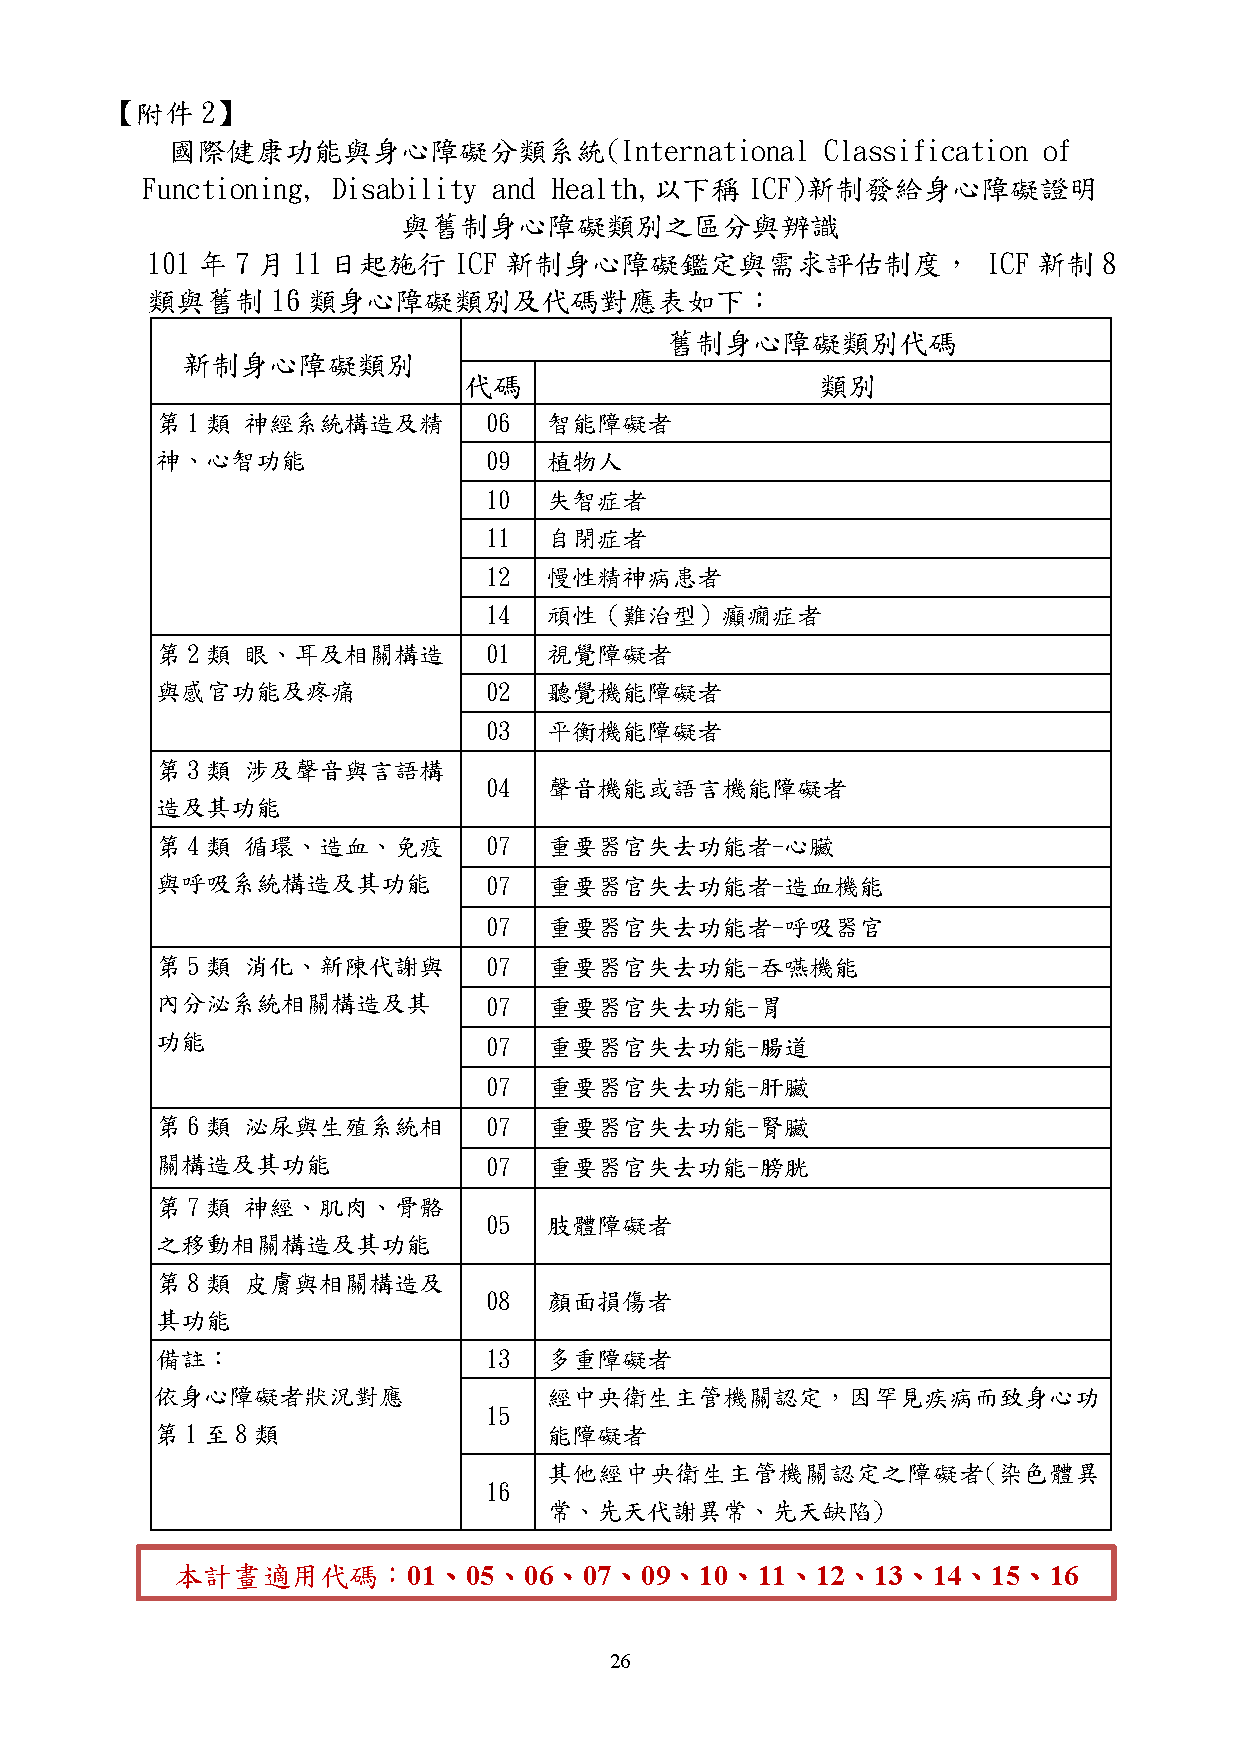
\includepdf[pages=-]{111年牙醫特殊醫療服務計畫 (ICF).pdf}

% 111年度申請補助作業規定_一般醫院 (綜合資料表).pdf
%\includepdf[pages=-]{}

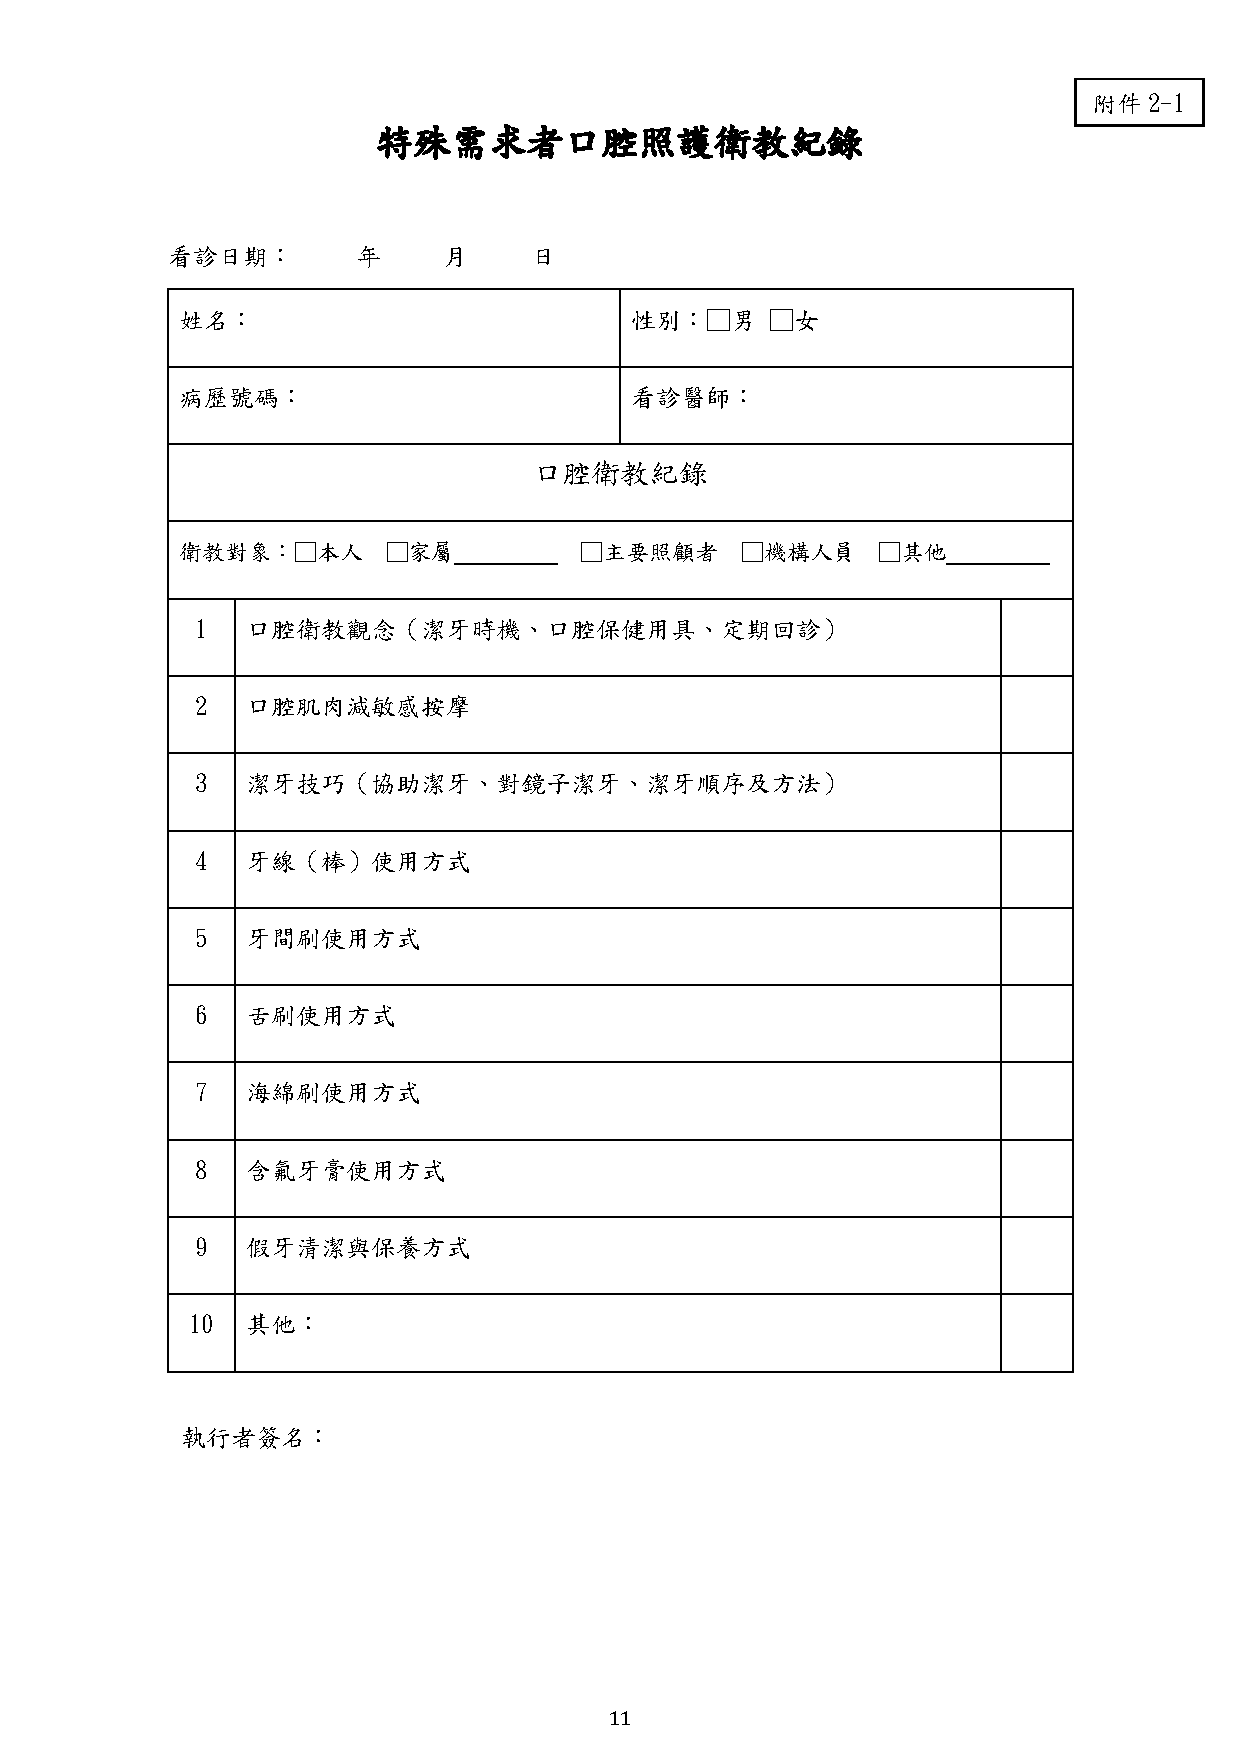
\includepdf[pages=-]{content/111年度申請補助作業規定_一般醫院 (附件 2-1).pdf} % (附件6)
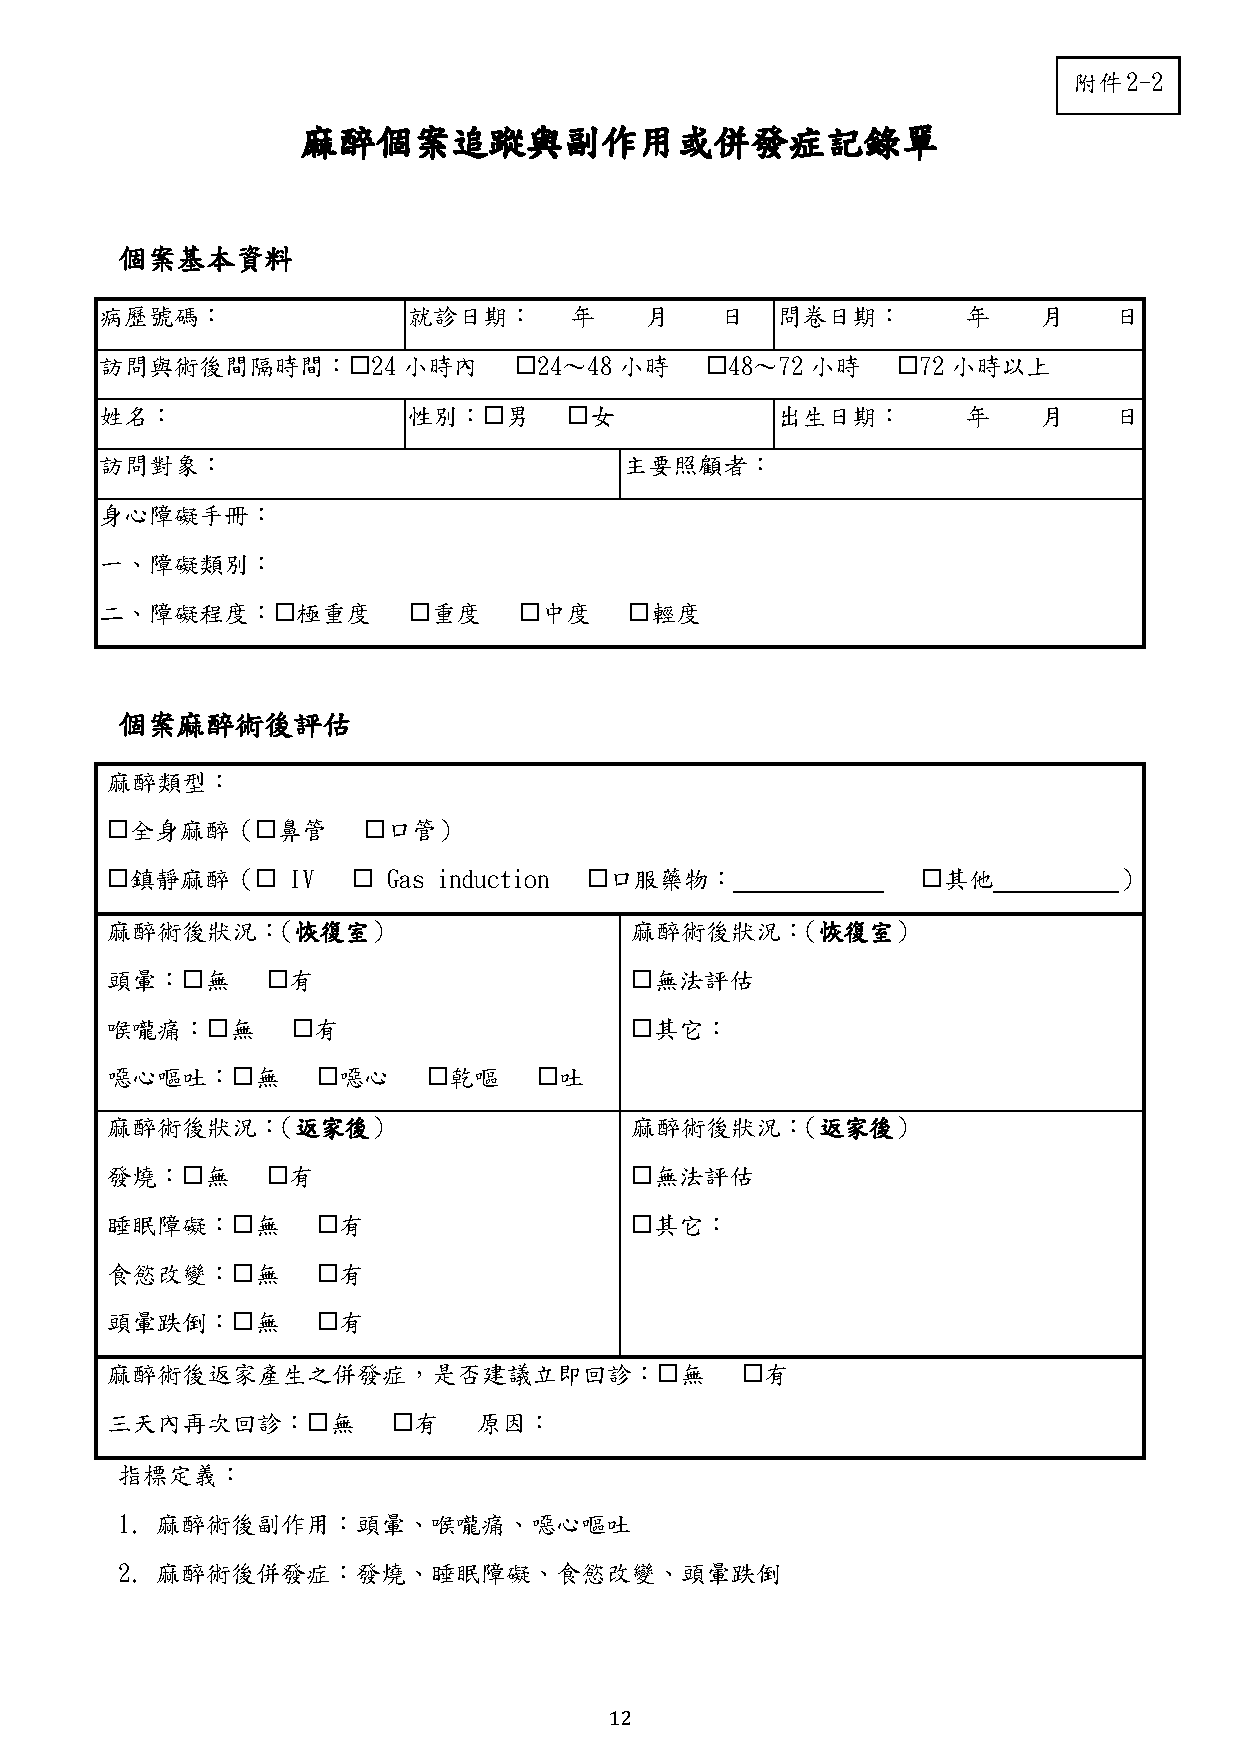
\includepdf[pages=-]{content/111年度申請補助作業規定_一般醫院 (附件 2-2).pdf} % (附件6)
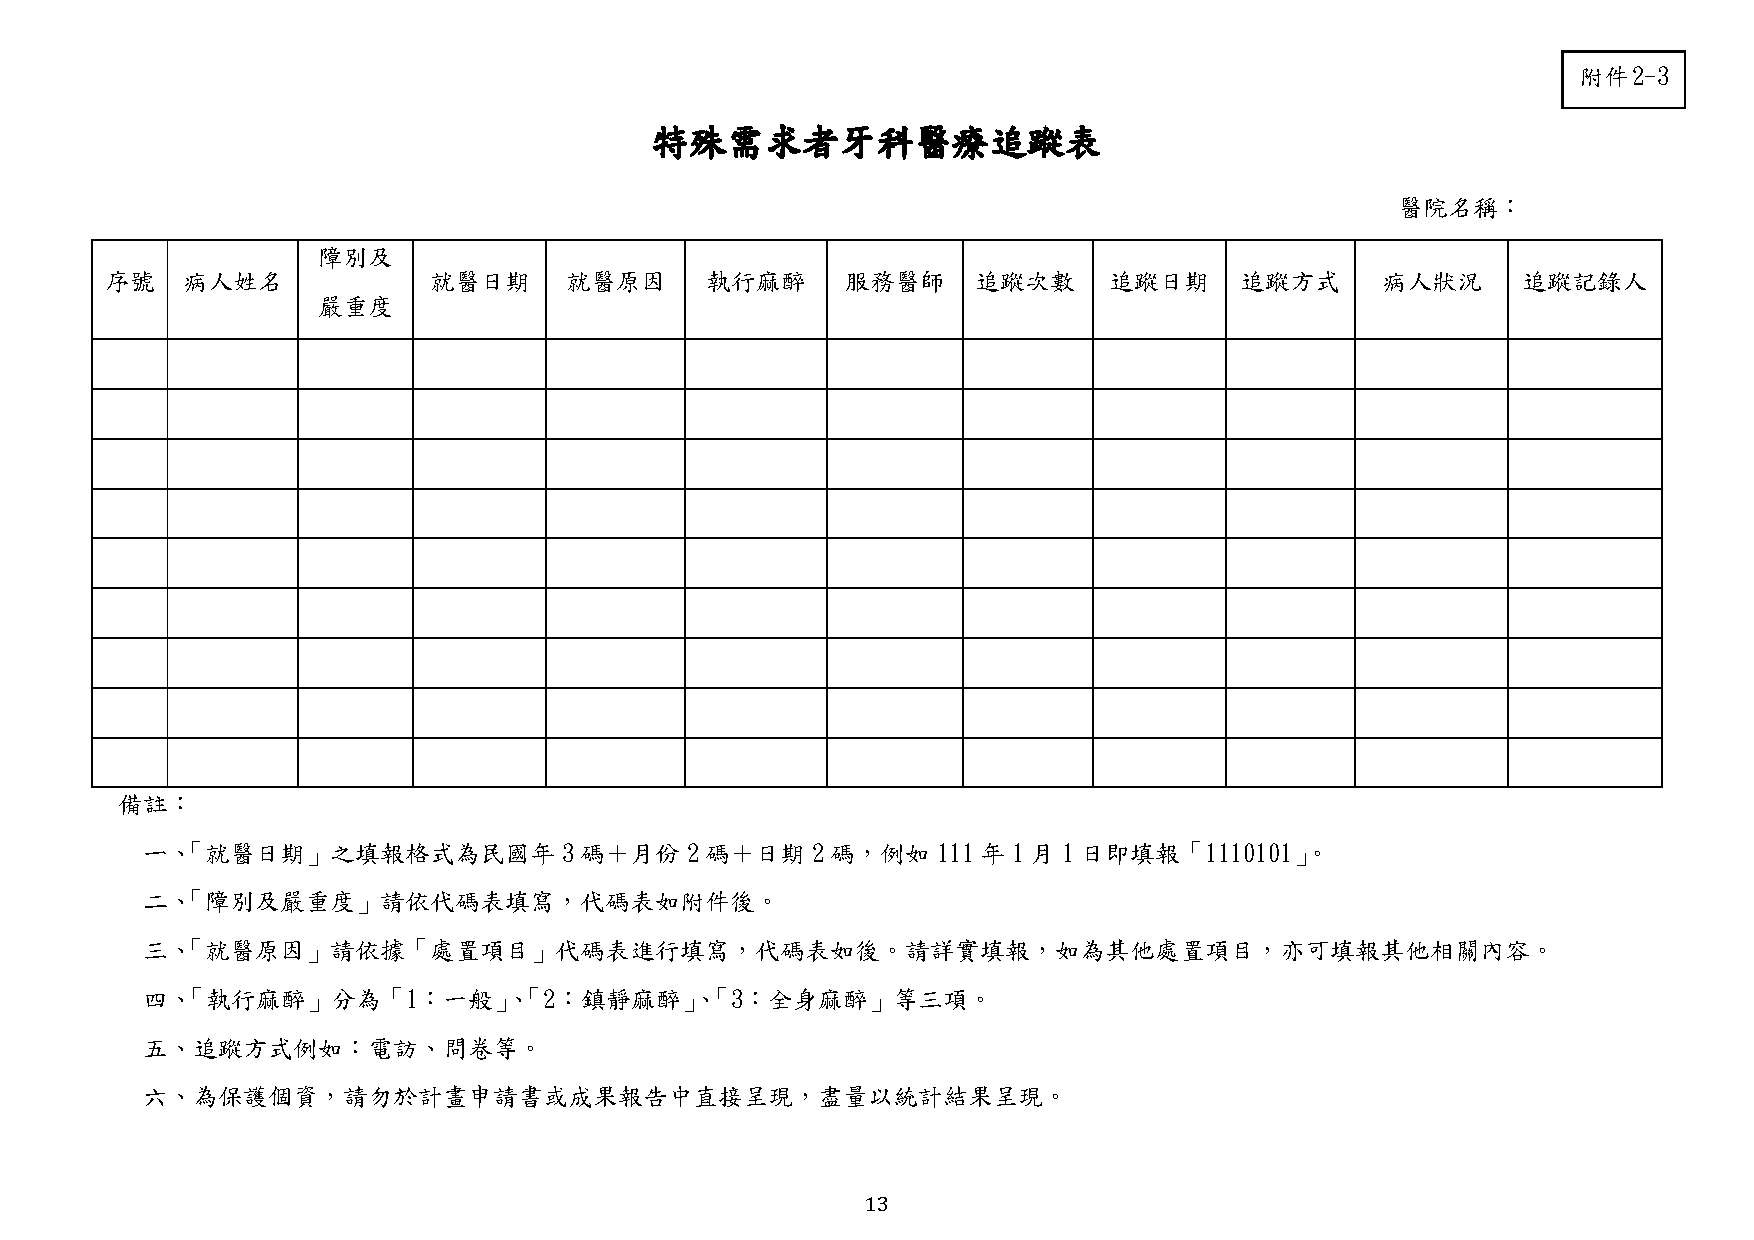
\includepdf[pages=-]{content/111年度申請補助作業規定_一般醫院 (附件 2-3).pdf} % (附件6)
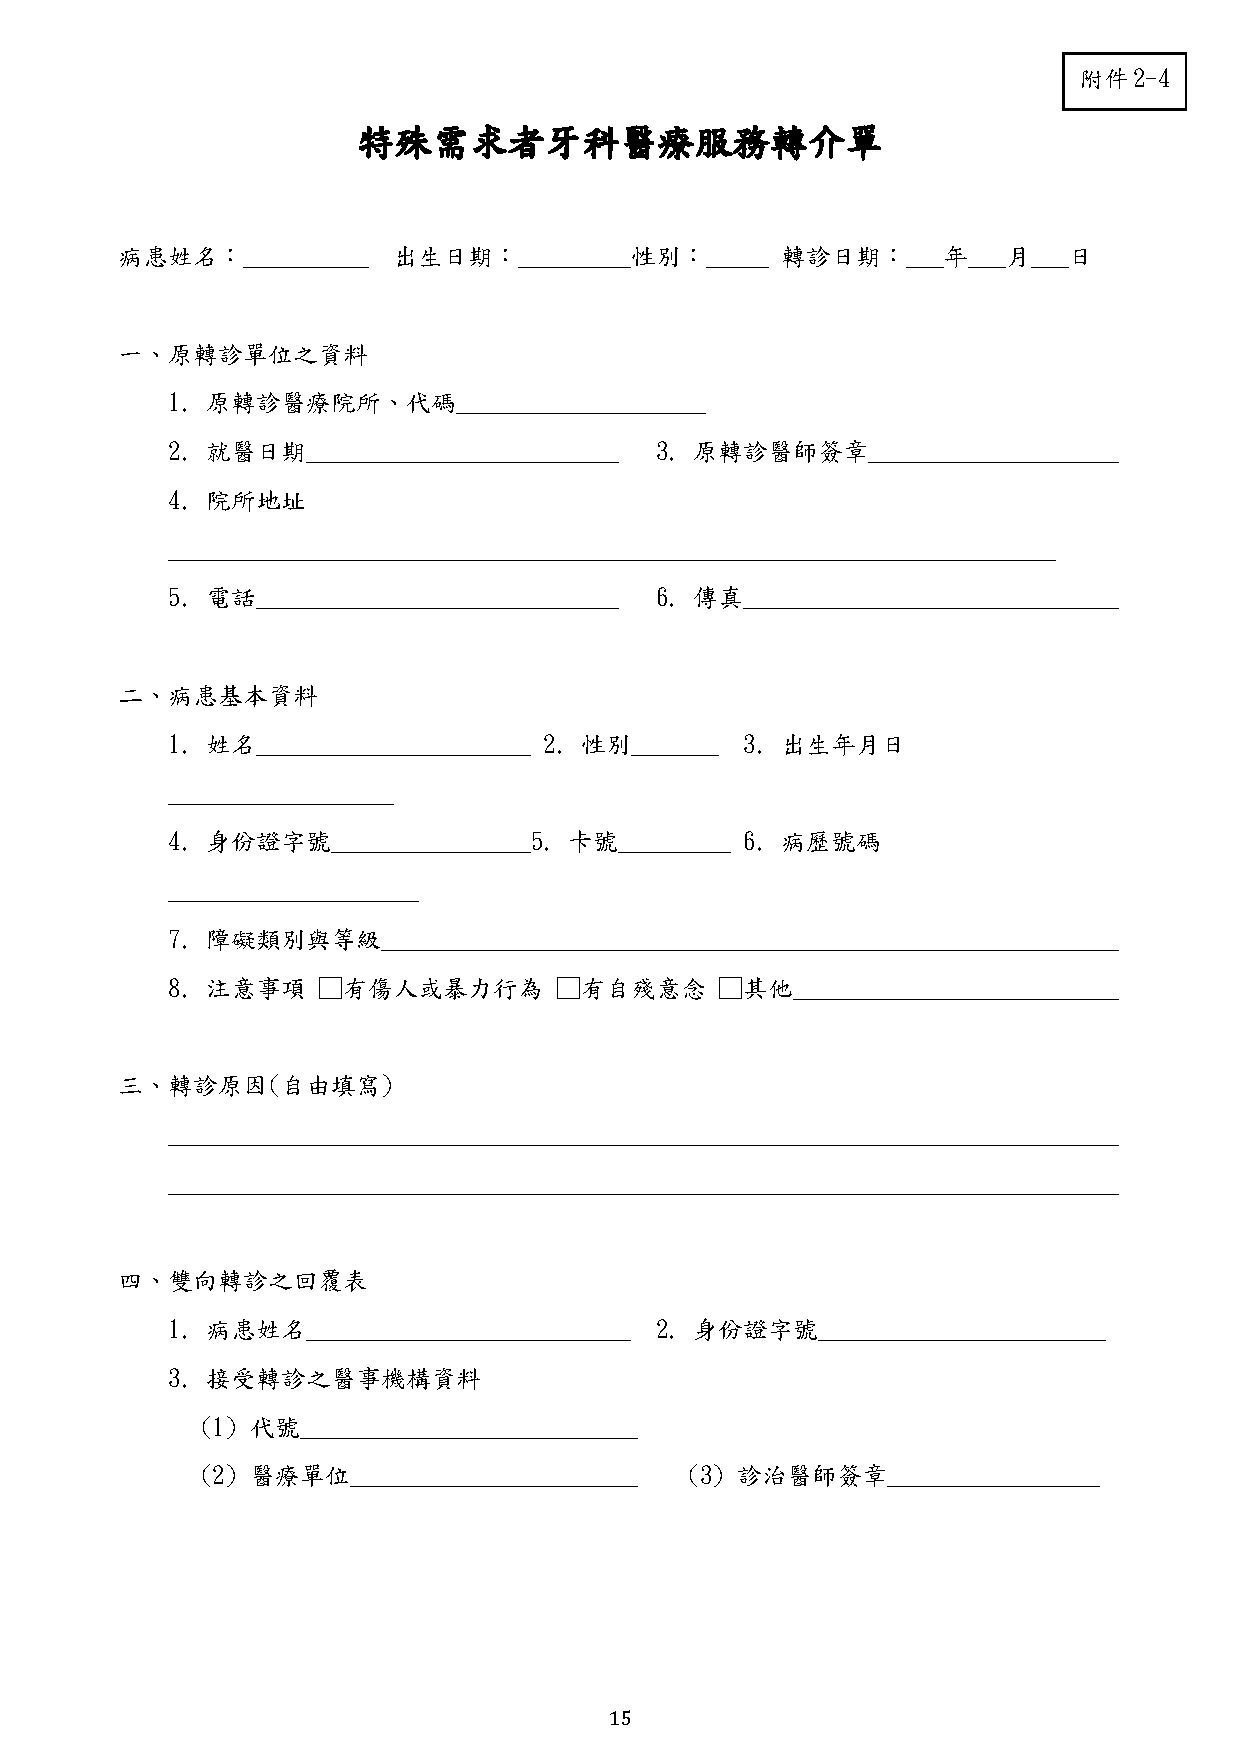
\includepdf[pages=-]{content/111年度申請補助作業規定_一般醫院 (附件 2-4).pdf} % (附件6)
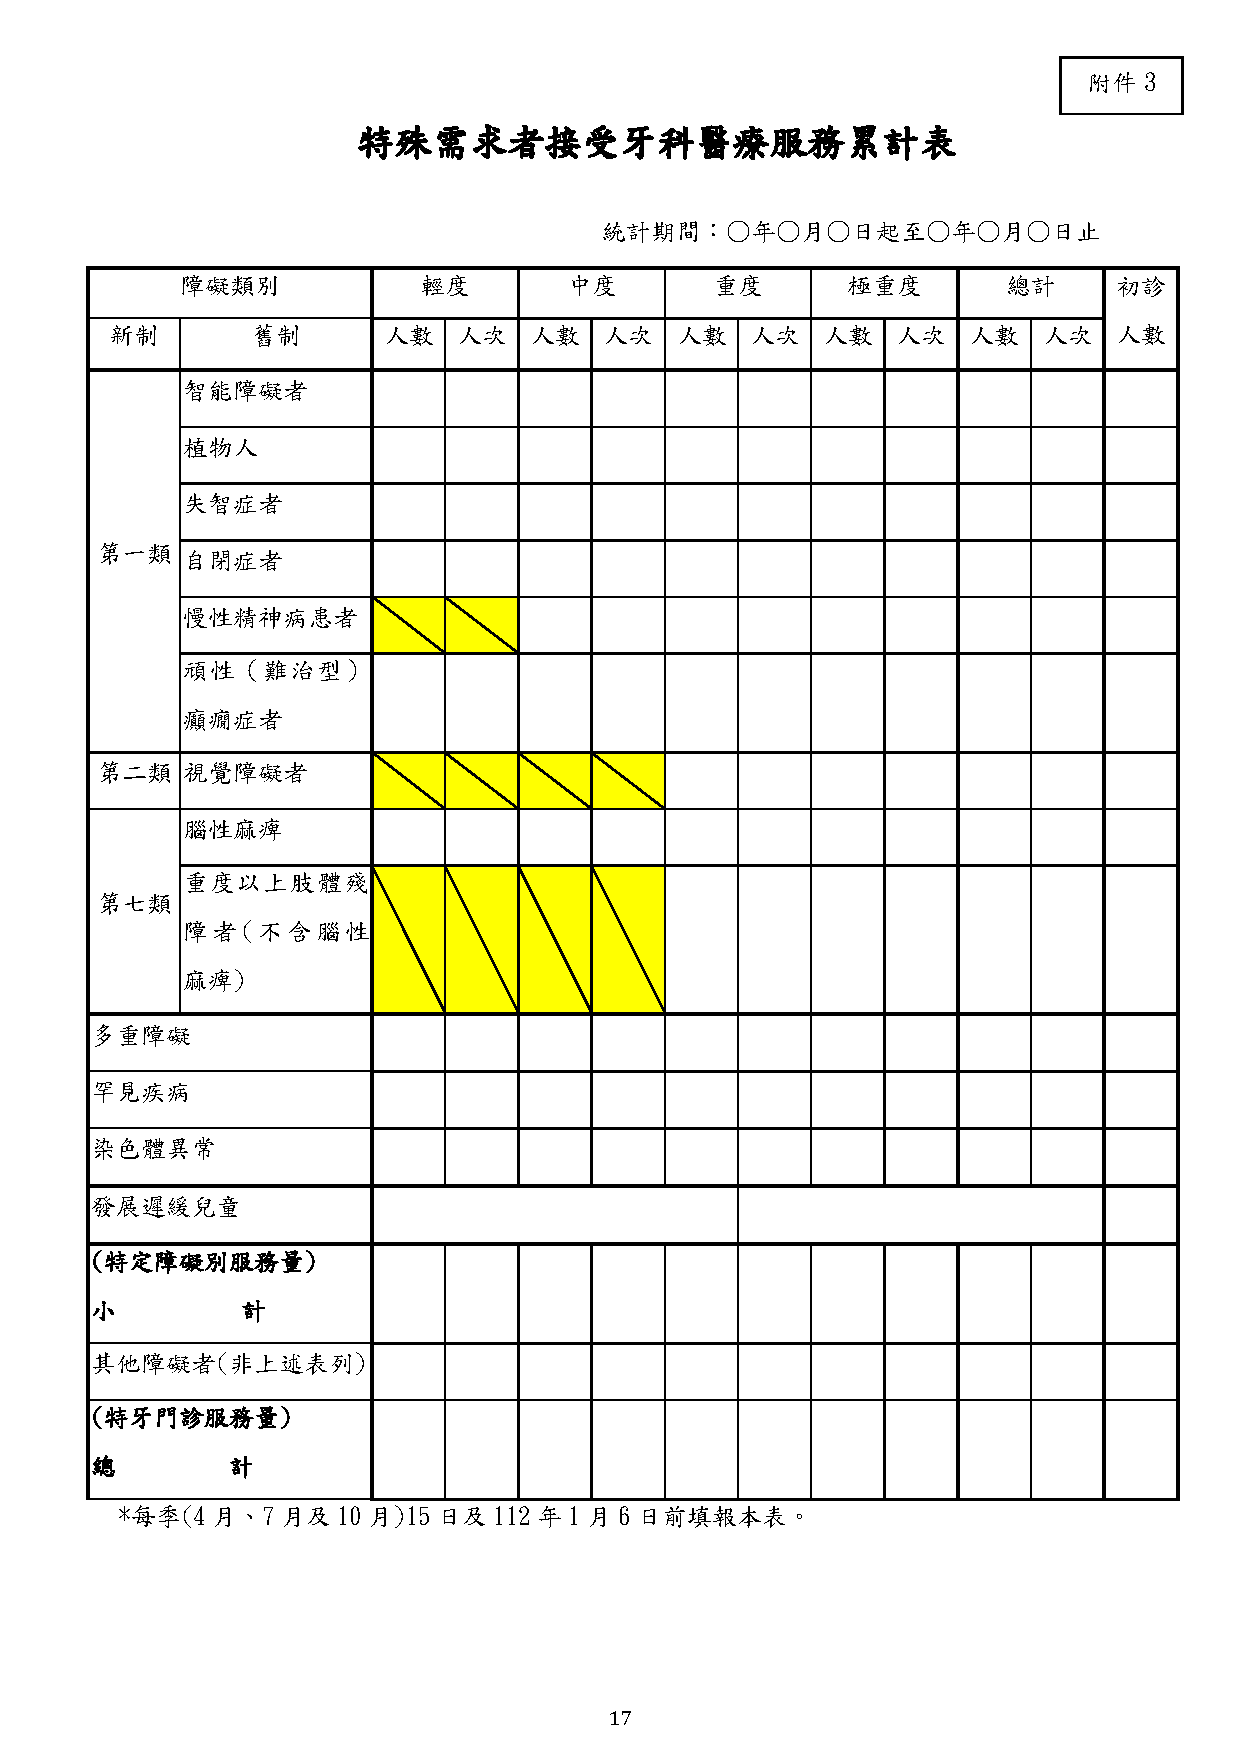
\includepdf[pages=-]{content/111年度申請補助作業規定_一般醫院 (附件 3).pdf} % (附件6)
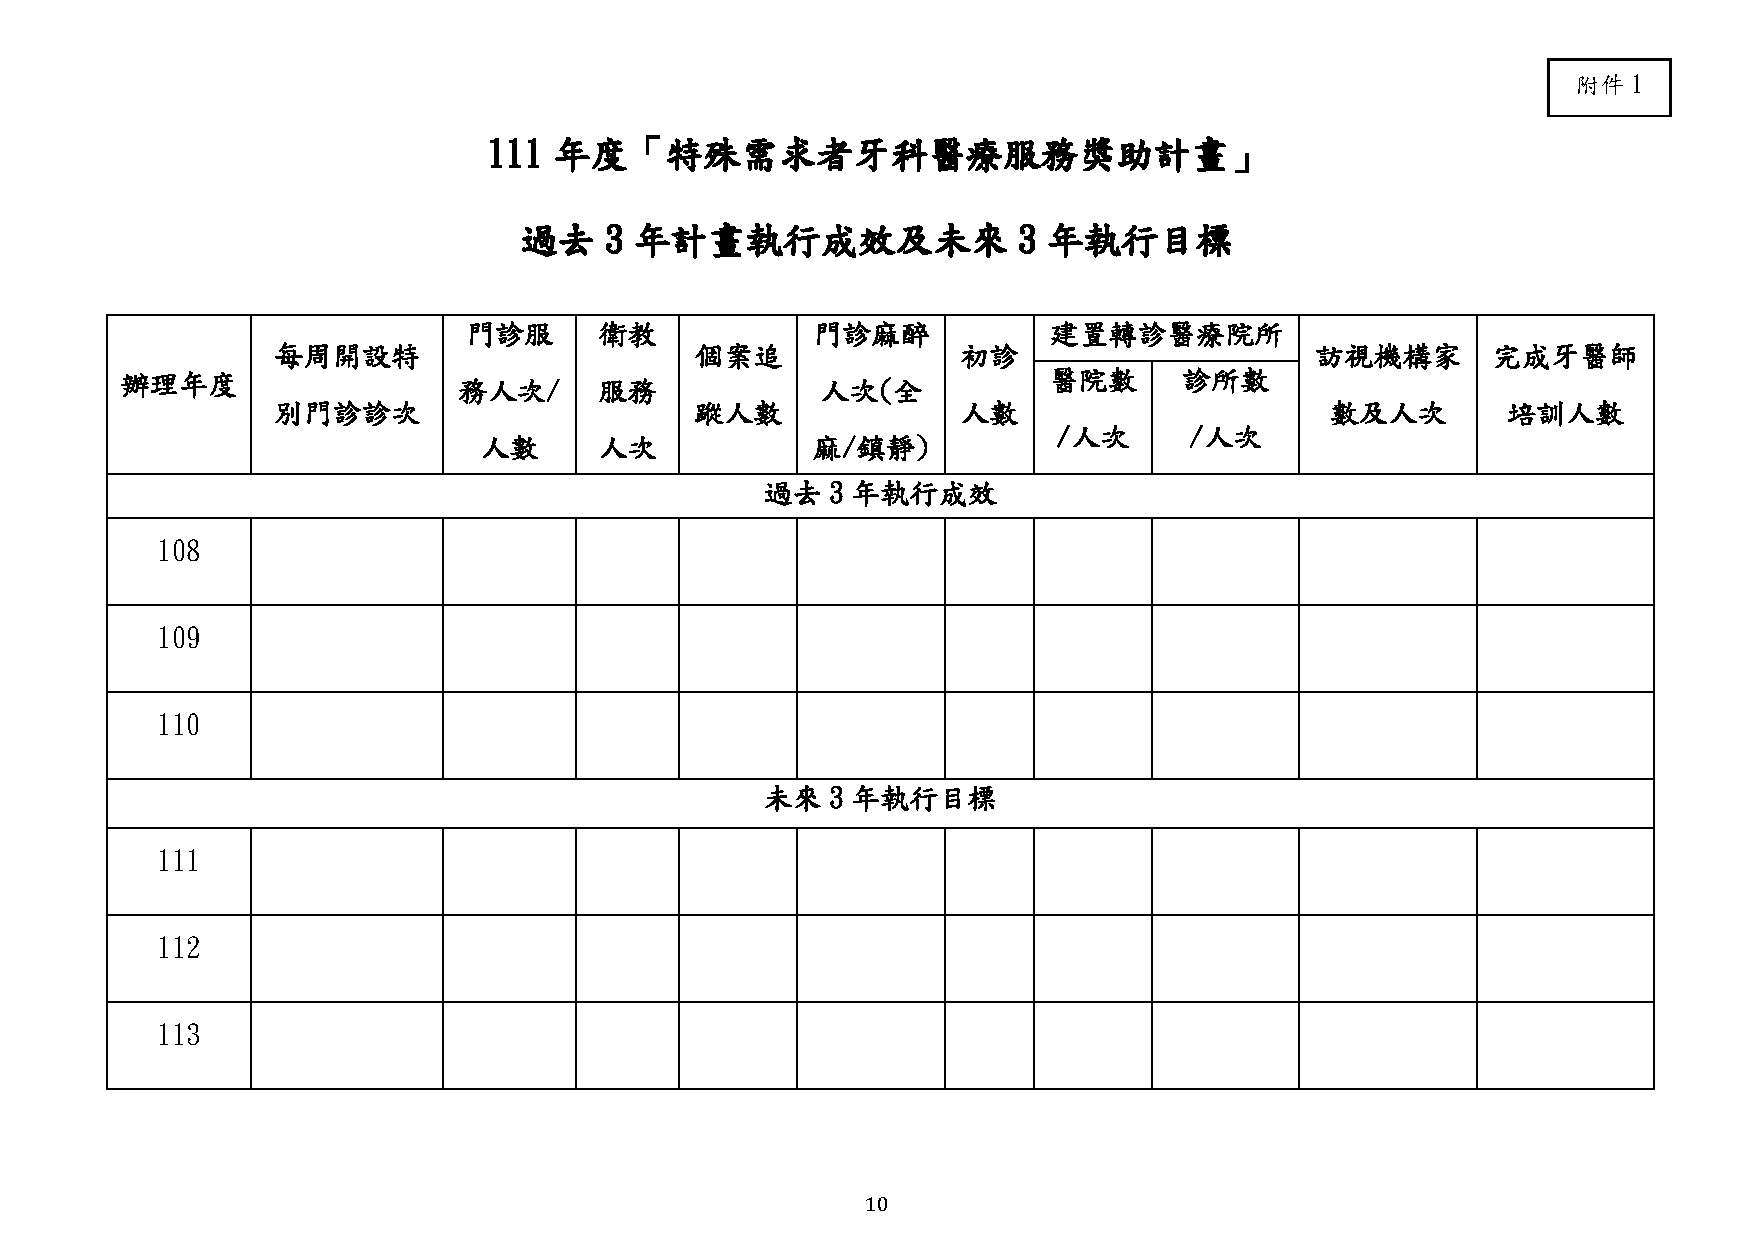
\includepdf[pages=-]{content/111年度申請補助作業規定_一般醫院 (附件 1).pdf} % (附件6)
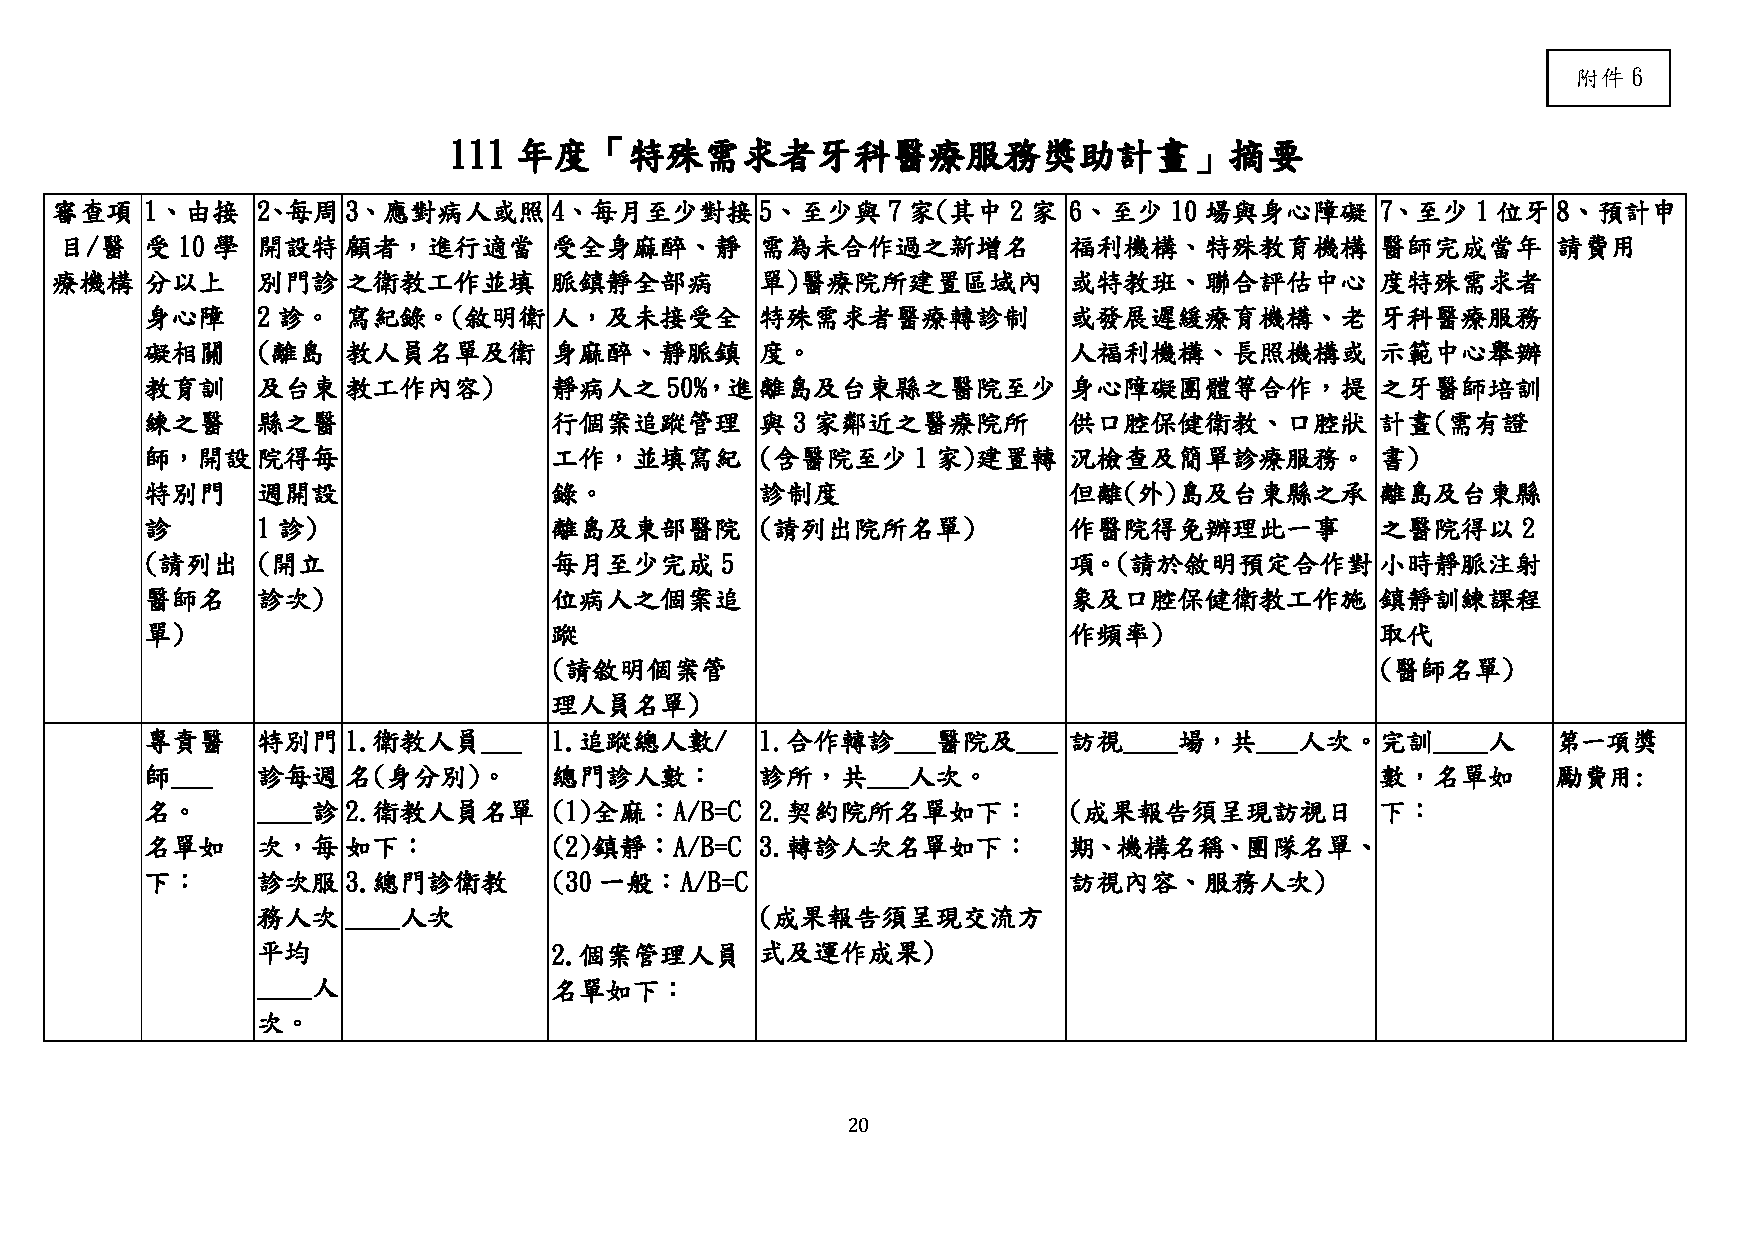
\includepdf[pages=-]{content/111年度申請補助作業規定_一般醫院 (summary 附件6).pdf} % (附件6)
\clearpage

%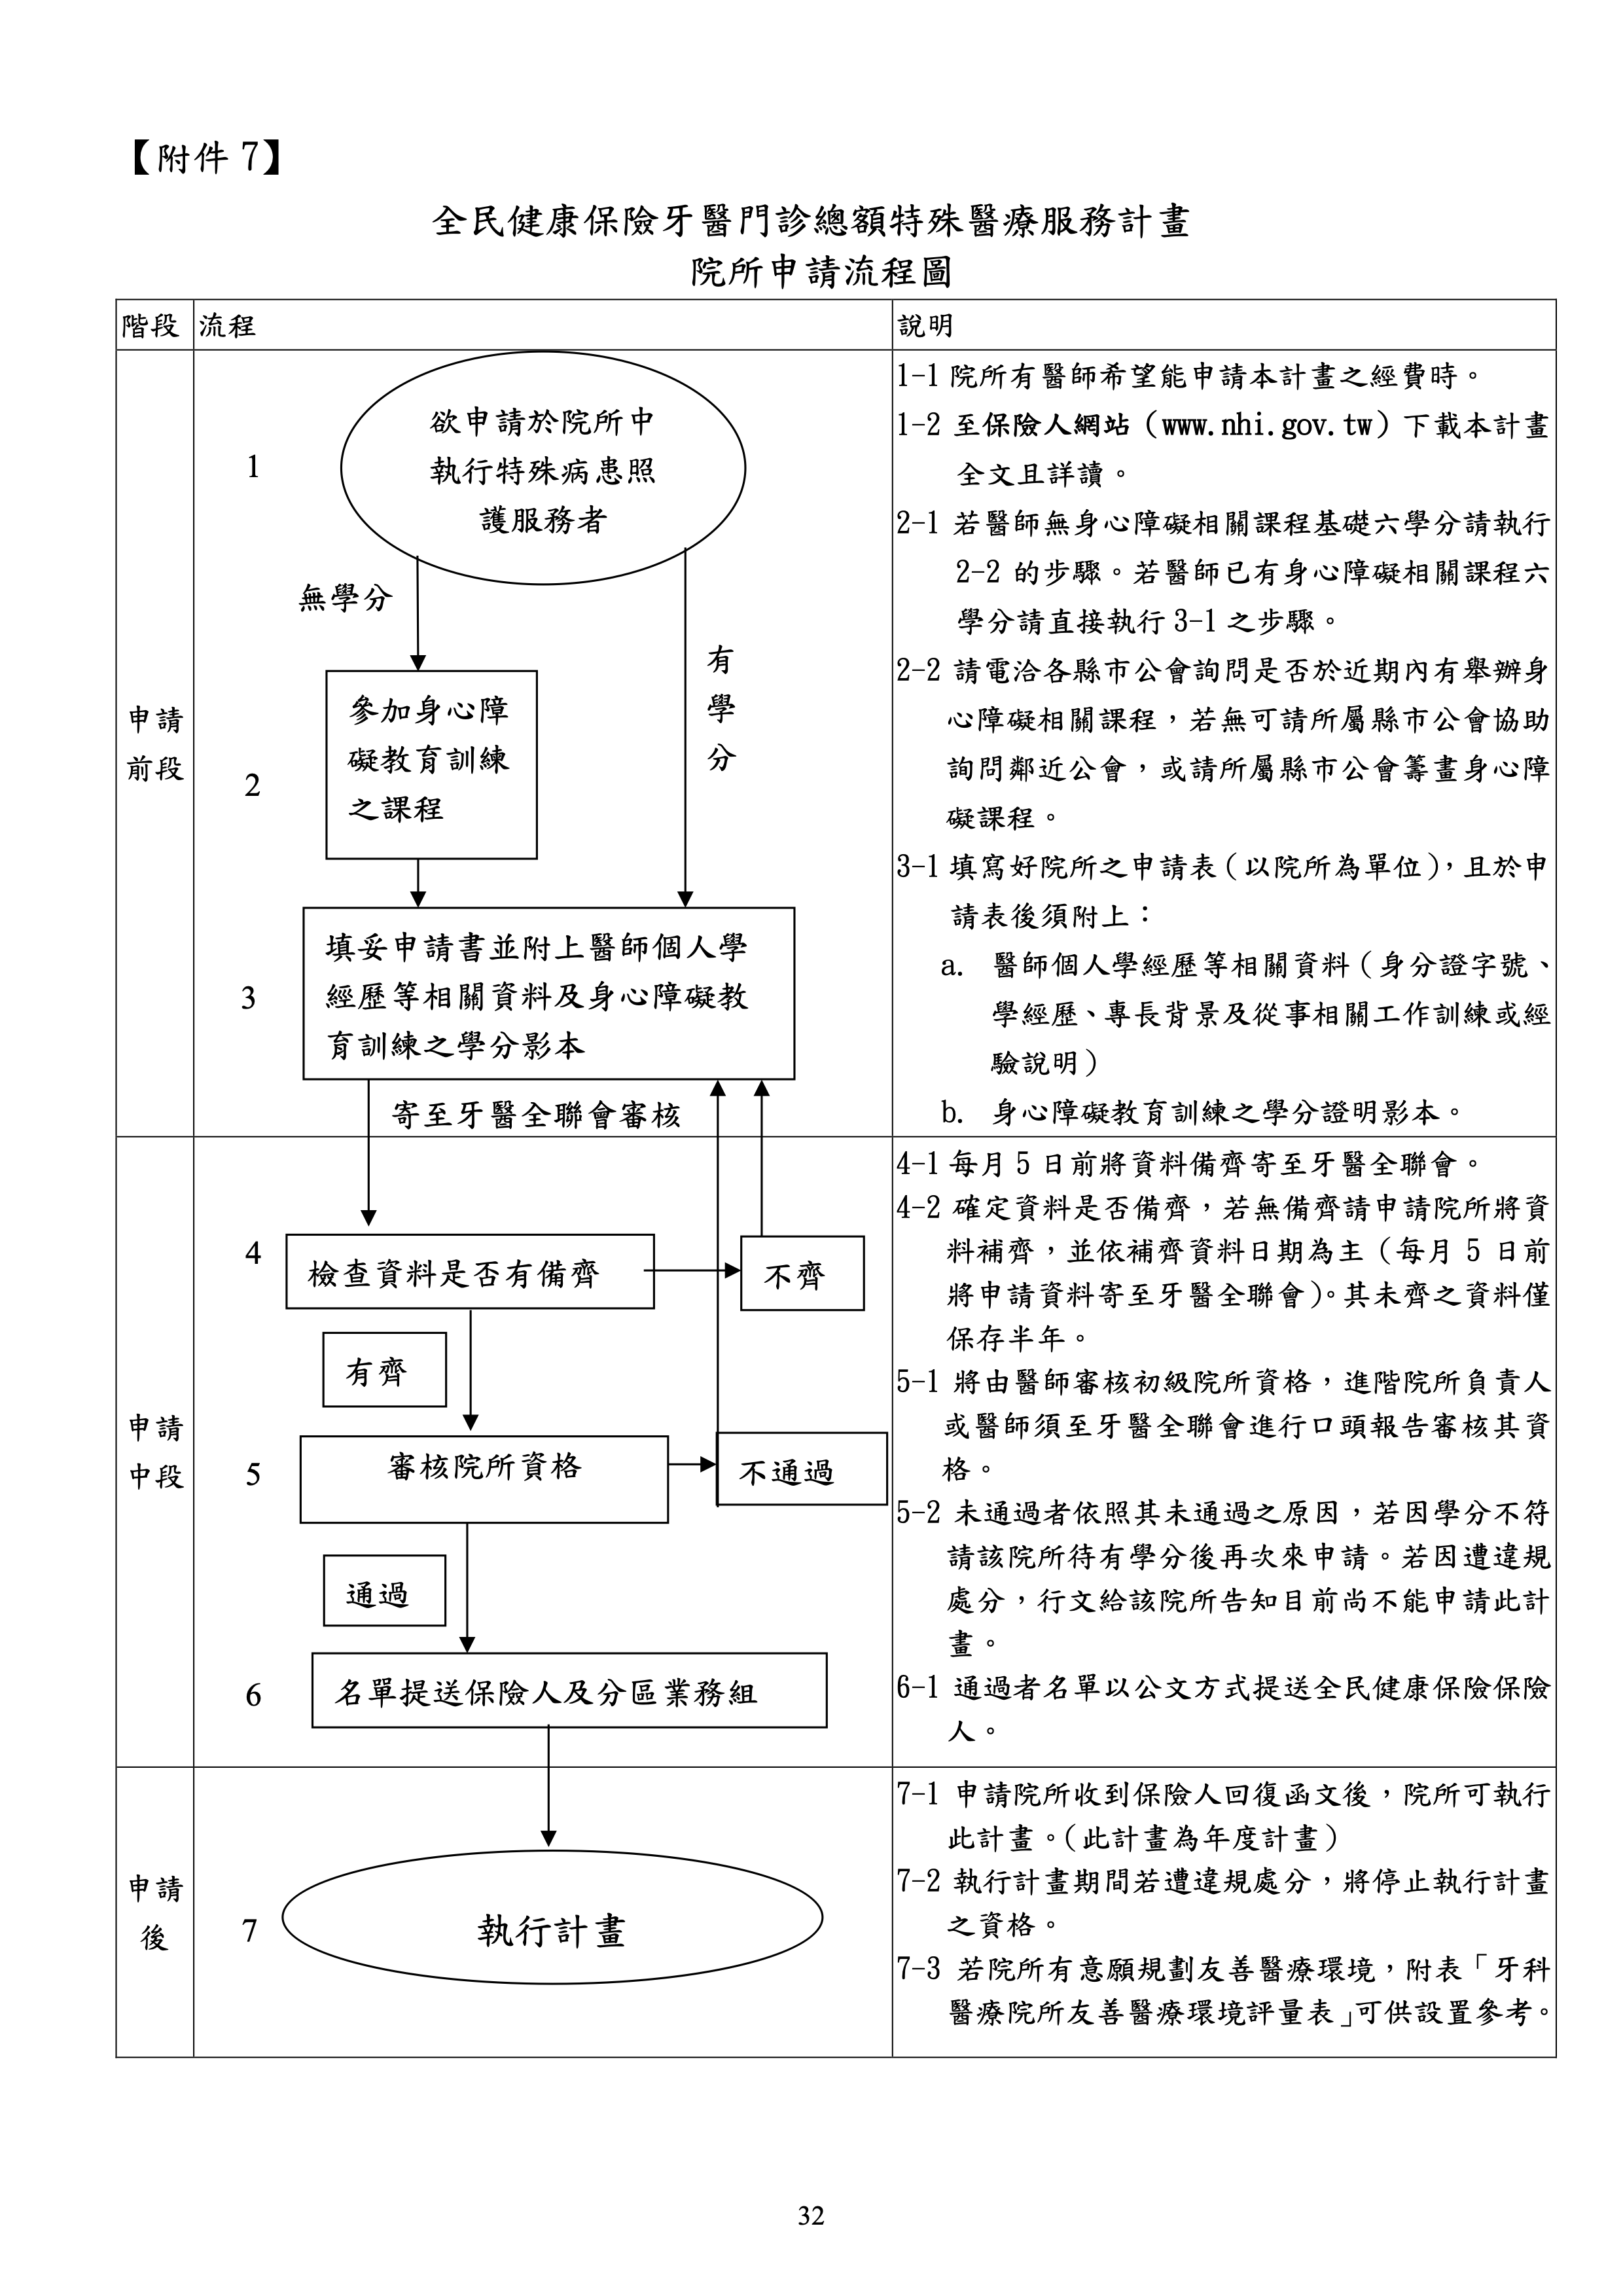
\includegraphics[width=0.9\textwidth]{111年牙醫特殊醫療服務計畫 (附件7).png}


%% Please add the following required packages to your document preamble:
% \usepackage{graphicx}

【附件19】

\begin{table}[H]
%\caption{}
%\label{tab:DOH_acls}
\centering
\resizebox{\textwidth}{!}{%
\begin{tabular}{|l|l|l|l|}
\hline
分類       & 名稱                           & 功能                                                                   & 備註      \\ \hline
BLS &
  Vital sign monitor &
  \begin{tabular}[c]{@{}l@{}}NIBP blood pressure (sphygmomanometer),\\ pulse oximeter (oxygen saturation, SpO2), pulse rate, BPM\end{tabular} &
  HP/Phillip \\ \hline
       & Glucose Meter                & blood sugar from finger tip                                          &         \\ \hline
       & Stethoscope                  & 心臟科聽診器                                                               &         \\ \hline
       & Oxygen supply                & ambu bag, face mask 6L/min; nasal prong (with cannula)               & O2 tank \\ \hline
       & Airway                       & nasopharyngeal airway (nasal trumpet, size #7 #8)                    &         \\ \hline
 &
  Airway (advance) &
  \begin{tabular}[c]{@{}l@{}}laryngeal mask airway (LMA), oral endotracheal tube (French #6, #7)\\ laryngoscope (插管用喉鏡 curved blade)/Magi forceps + Lidocaine jelly\end{tabular} &
   \\ \hline
Drug   & Allergy with broncospasm     & 肌肉內注射 0.2-0.5mg epinephrine (1 mg/mL)                                &         \\ \hline
       & Status epilepticus (> 5 min) & diazepam 肌肉或靜脈注射(靜脈注射較佳),初劑量 5-10mg                                  &         \\ \hline
Dental & 攜帶式超音波洗牙機                    & NSK Varios 970 LUX (water supply, fibroptic cable)                   &         \\ \hline
       & 攜帶式真空吸引機(suction machine)    & 抽痰管, suction tip with saliva ejector, 治療巾, 彎盆                        &         \\ \hline
       & PPE                          & 口罩surgical mask 隔離衣gown 護目鏡goggle                                    & x3      \\ \hline
       & Fluoridation                 & 氟膠 Sodium Fluoride gel 5\%(Clinpro[3M] vanish with brush), 2x2 gauze &         \\ \hline
 &
  衛教 &
  \begin{tabular}[c]{@{}l@{}}張口棒(健康牌)、木質壓舌板、\\ 兒童牙刷(soft brush, flat handle)、牙間刷、3M牙線棒\end{tabular} &
   \\ \hline
       & 感控                           & 75\% alcohol swab、乾洗手液,檢診手套,紅色感染用塑膠袋                                 &         \\ \hline
Others &                              & 手電筒, 電源延長線/adaptor                                                   &         \\ \hline
\end{tabular}%
}

\end{table} % 附件19

\end{document}
